\documentclass[11pt]{article}
\setlength\headheight{13.6pt}%
\usepackage[utf8]{inputenc} % Required for inputting international characters
\usepackage[T1]{fontenc} % Output font encoding for international characters
\usepackage{polski}
\usepackage{mathpazo} % Palatino font
\usepackage{graphicx}
\usepackage{fancyhdr}
\usepackage{etoolbox}
\usepackage{blindtext}
\usepackage{geometry}
\geometry{legalpaper, margin=1in}
\usepackage[cleardoublepage=plain]{scrextend}
\graphicspath{ {images/C:\Users\Kuba-PC\Desktop\ProjektIO} }
\pagestyle{fancy}
\fancyhf{}
\rhead{2017/2018}
\lhead{Projekt z Inżynierii Oprogramowania}
\rfoot{Strona \thepage}
\begin{document}
	
	\begin{titlepage} 
	
		\newcommand{\HRule}{\rule{\linewidth}{0.5mm}} % Defines a new command 
		
		\center % Centre everything on the page
		
		%------------------------------------------------
		%	Nagłówki
		%------------------------------------------------
		
		\textsc{\LARGE Akademia Górniczo-Hutnicza im. Stanisława Staszica w Krakowie}\\[1.5cm] % Main heading such as the name of your university/college
		
		\textsc{\Large Projekt z Inżynierii Oprogramowania}\\[0.5cm] % Major heading such as course name
		
		\textsc{\large Informatyka EAIiB 2017/2018}\\[0.5cm] % Minor heading such as course title
		
		%------------------------------------------------
		%	Tytuł
		%------------------------------------------------
		
		\HRule\\[0.4cm]
		
		{\huge\bfseries Lokalizacja w pomieszczeniach bez użycia sygnału GPS}\\[0.4cm] % Title of your document
		
		\HRule\\[1.5cm]
		
		%------------------------------------------------
		%	Authorzy
		%------------------------------------------------
		
		\begin{minipage}{0.4\textwidth}
			\begin{flushleft}
				\large
				\textit{Autorzy}\\
				Jakub \textsc{Kacorzyk} \\
				Bartłomiej \textsc{Łazarczyk}
			\end{flushleft}
		\end{minipage}
		~
		\begin{minipage}{0.4\textwidth}
			\begin{flushright}
				\large
				\textit{Prowadzący}\\
				dr inż. Radosław \textsc{Klimek} % Supervisor's name
			\end{flushright}
		\end{minipage}
		
		%------------------------------------------------
		%	Logo
		%------------------------------------------------
		
		\vfill\vfill
		
\includegraphics[scale=0.5]{logo.jpg}
		
		%------------------------------------------------
		%	Data
		%------------------------------------------------
		
		\vfill\vfill\vfill % Position the date 3/4 down the remaining page
		
		{\large\today} 
		
		%----------------------------------------------------------------------------------------
		
		\vfill % Push the date up 1/4 of the remaining page
		
	\end{titlepage}
	
	\tableofcontents
	\cleardoublepage
	\setcounter{page}{2}
	
	
	\section{Streszczenie}
	Projekt modeluje działanie aplikacji mobilnej lokalizującej użytkownika w środowisku indoor. 
	Głównym założeniem systemu jest wyznaczenie oraz śledzenie lokalizacji klienta bez udziału sygnału GPS. Aby to osiągnąć wykorzystywane są urządzenia dostępu do sieci Wi-Fi znajdujące się w budynku, maszty telefonii komórkowej oraz urządzenia pomiarowe dostępne w telefonie takie jak akcelerometr, magnetometr, barometr.
	
	Wyznaczanie pozycji startowej zależy od dostępu do internetu oraz otaczających sieci Wi-Fi.
	W przypadku niespełnienia powyższych warunków wyznaczany jest potencjalny obszar na podstawie informacji uzyskanych z sieci komórkowej. Im więcej nadajników sieci komórkowej użytkownika w pobliżu, tym dokładniejszy jest wyznaczony obszar.
	Po ustaleniu pozycji bazowej, aplikacja opiera się na urządzeniach pomiarowych dostępnych  w telefonie do śledzenia zmiany jego położenia. W przypadku otrzymania kolejnej informacji od urządzenia zewnętrznego, porównywana jest ona ze zmianami zarejestrowanymi przez telefon oraz wyznaczany jest dopuszczalny błąd pomiarowy dla urządzenia które tą informację przesłało. Ostateczną lokalizację wyznacza specjalny algorytm na podstawie wszystkich uzyskanych w danym momencie danych.
	
	\section{Lista obiektów}
	\begin{itemize}
		\item Wi-Fi
		\item Aplikacja mobilna
		\item Użytkownik
		\item Barometr
		\item Akcelerometr
		\item Magnetometr
		\item Maszty telefonii komórkowej
	\end{itemize}
	
	\section{Lista bodźców}
	\begin{itemize}
		\item Sygnały taktowane zegarem
		\begin{enumerate}
			
		\item Żądanie udostępnienia informacji o urządzeniu punktu dostępu wi-fi oraz o otrzymywanym sygnale
	    \item Żądanie określenia lokalizacji wysyłane przez aplikację mobilną
		\item Żądanie wyznaczenia kierunku przez magnetometr
		\item Żądanie wyznaczenia ciśnienia przez barometr
		\item Żądanie wyznaczenia zmiany prędkości przez akcelerometr
		
		\end{enumerate}
		\item Sygnały sterujące
		\begin{enumerate}
		\item Zlecenie lokalizacji urządzenia przez użytkownika
		\item Zlecenie wyznaczenia przebytej trasy przez użytkownika
		\item Zlecenie śledzenia lokalizacji przez użytkownika
	    \item Zwrócenie wyznaczonej trasy przez system obsługi lokalizacji
		\item Zwrócenie danych o położeniu  przez system obsługi lokalizacji
				
		\end{enumerate}
		\item Sygnały przepływu danych
		\begin{enumerate}
		\item	Dane o zmianach ciśnienia pobierane z barometra.
		\item	Dane o zmianach kierunku pobierane z magnetometra.
		\item	Dane położenia względem masztów telefonii komórkowej.
		\item	Dane o zmianach prędkości poruszania się pobierane z akcelerometra.
		\item	Dane o urządzeniu pobierane z urządzenia Wi-Fi
		\item	Dane o sygnale pobierane z urządania Wi-Fi
				
		\end{enumerate}
	\end{itemize}
	\newpage
	\section{Diagram kontekstowy}
    \begin{center}
	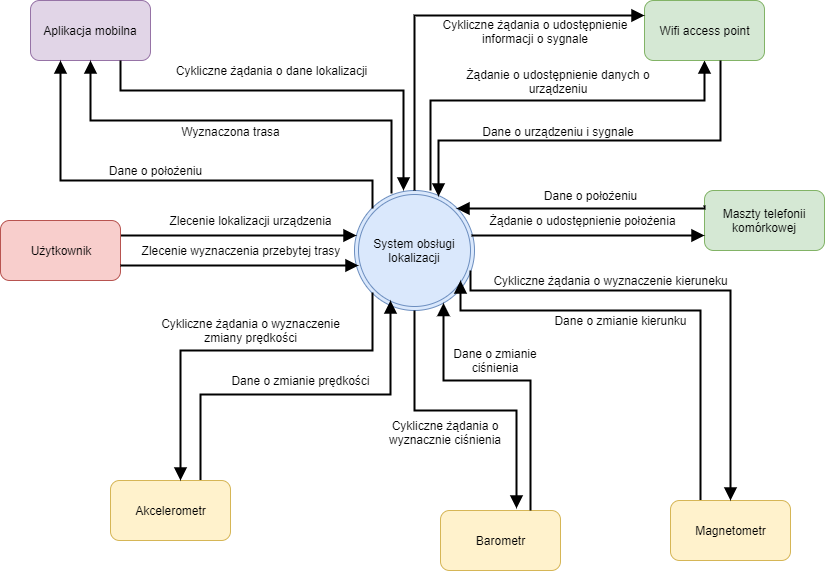
\includegraphics[scale=0.6]{DiagramKontekstowy.png}
	\end{center}
	\newpage
	\section{DFD poziom 0}
	\begin{center}
		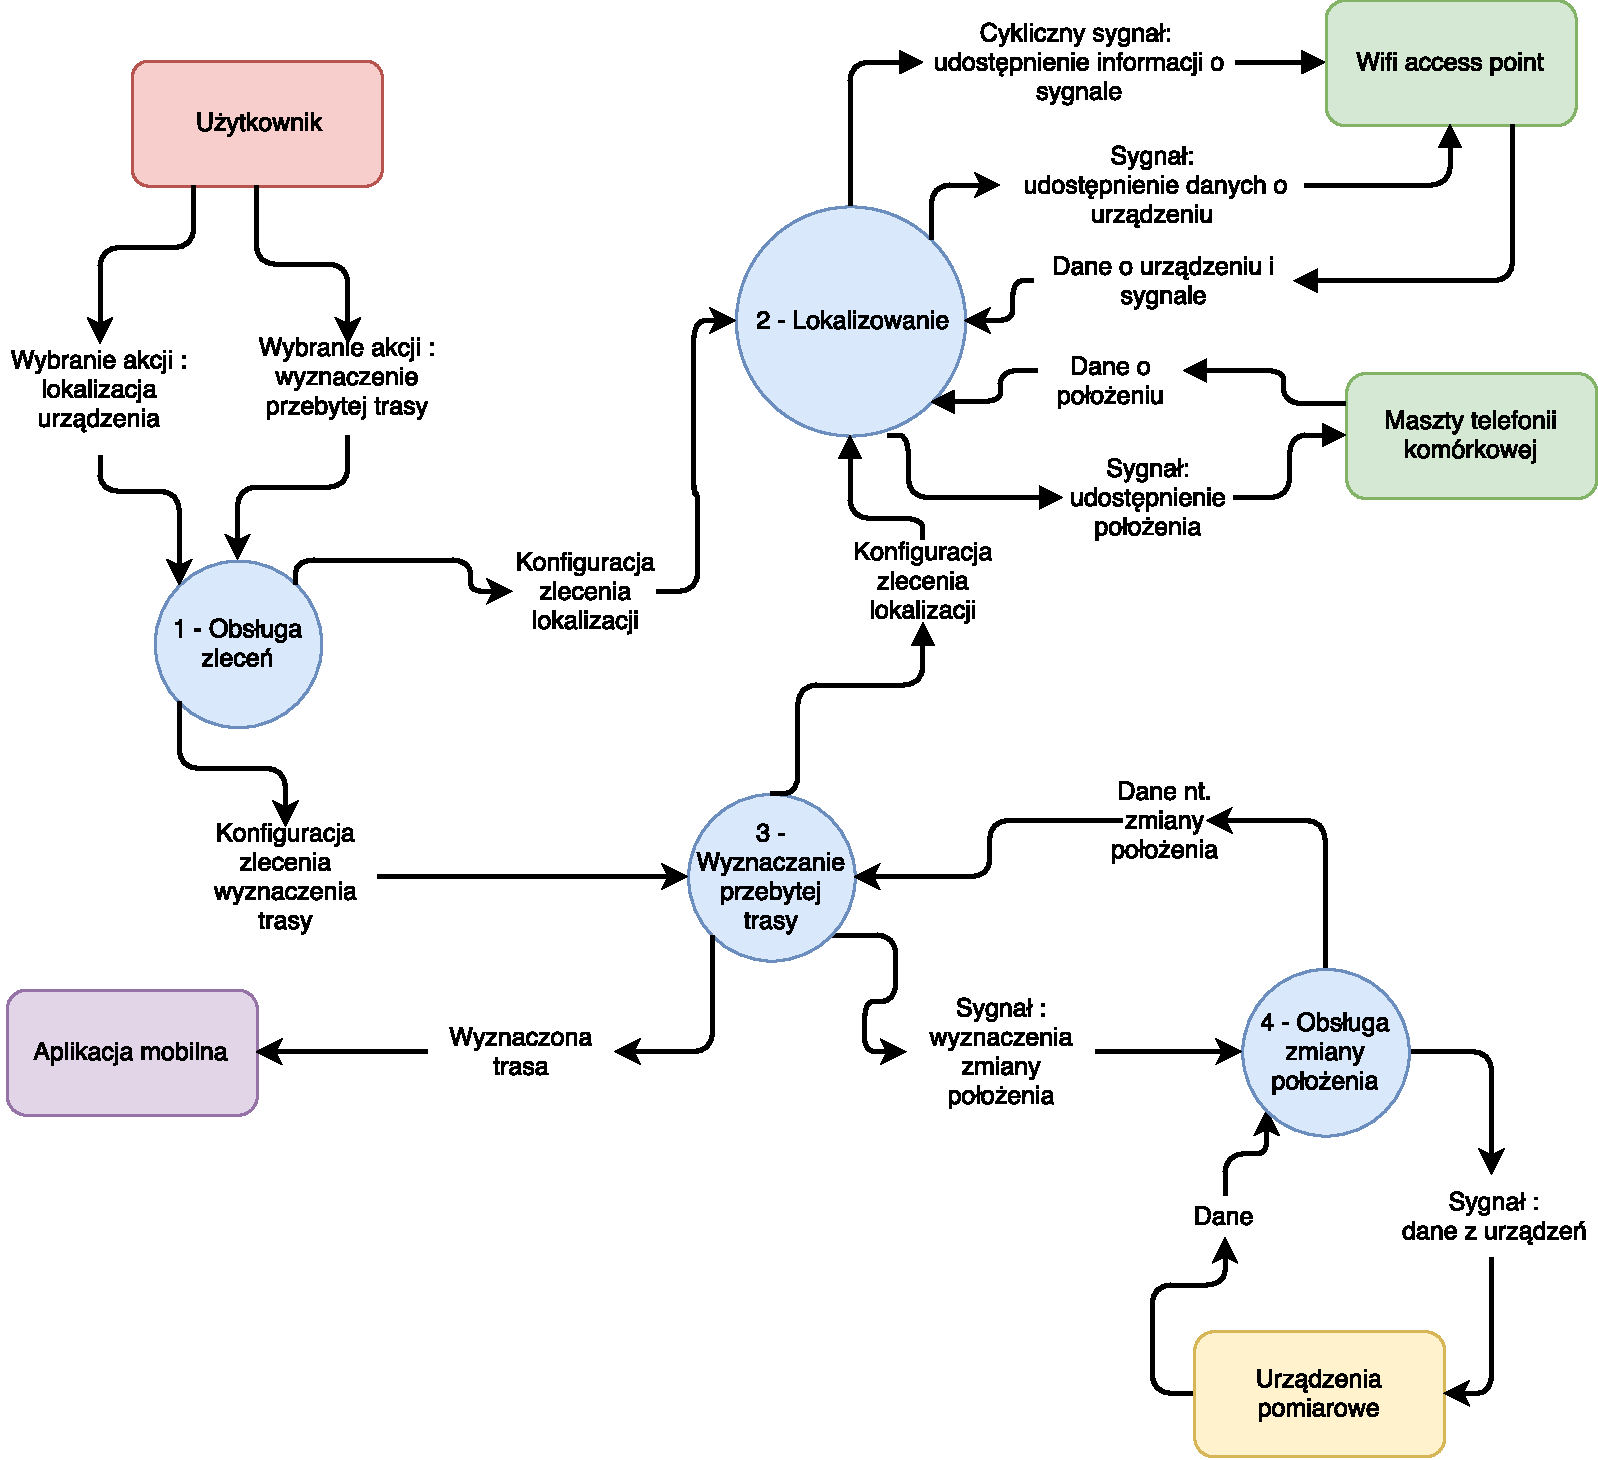
\includegraphics[scale=0.8]{DFD0.pdf}
	\end{center}
	\newpage
	\section{DFD poziom 1}
	\subsection{DFD poziom 1 - Osługa zleceń}
	\begin{center}
		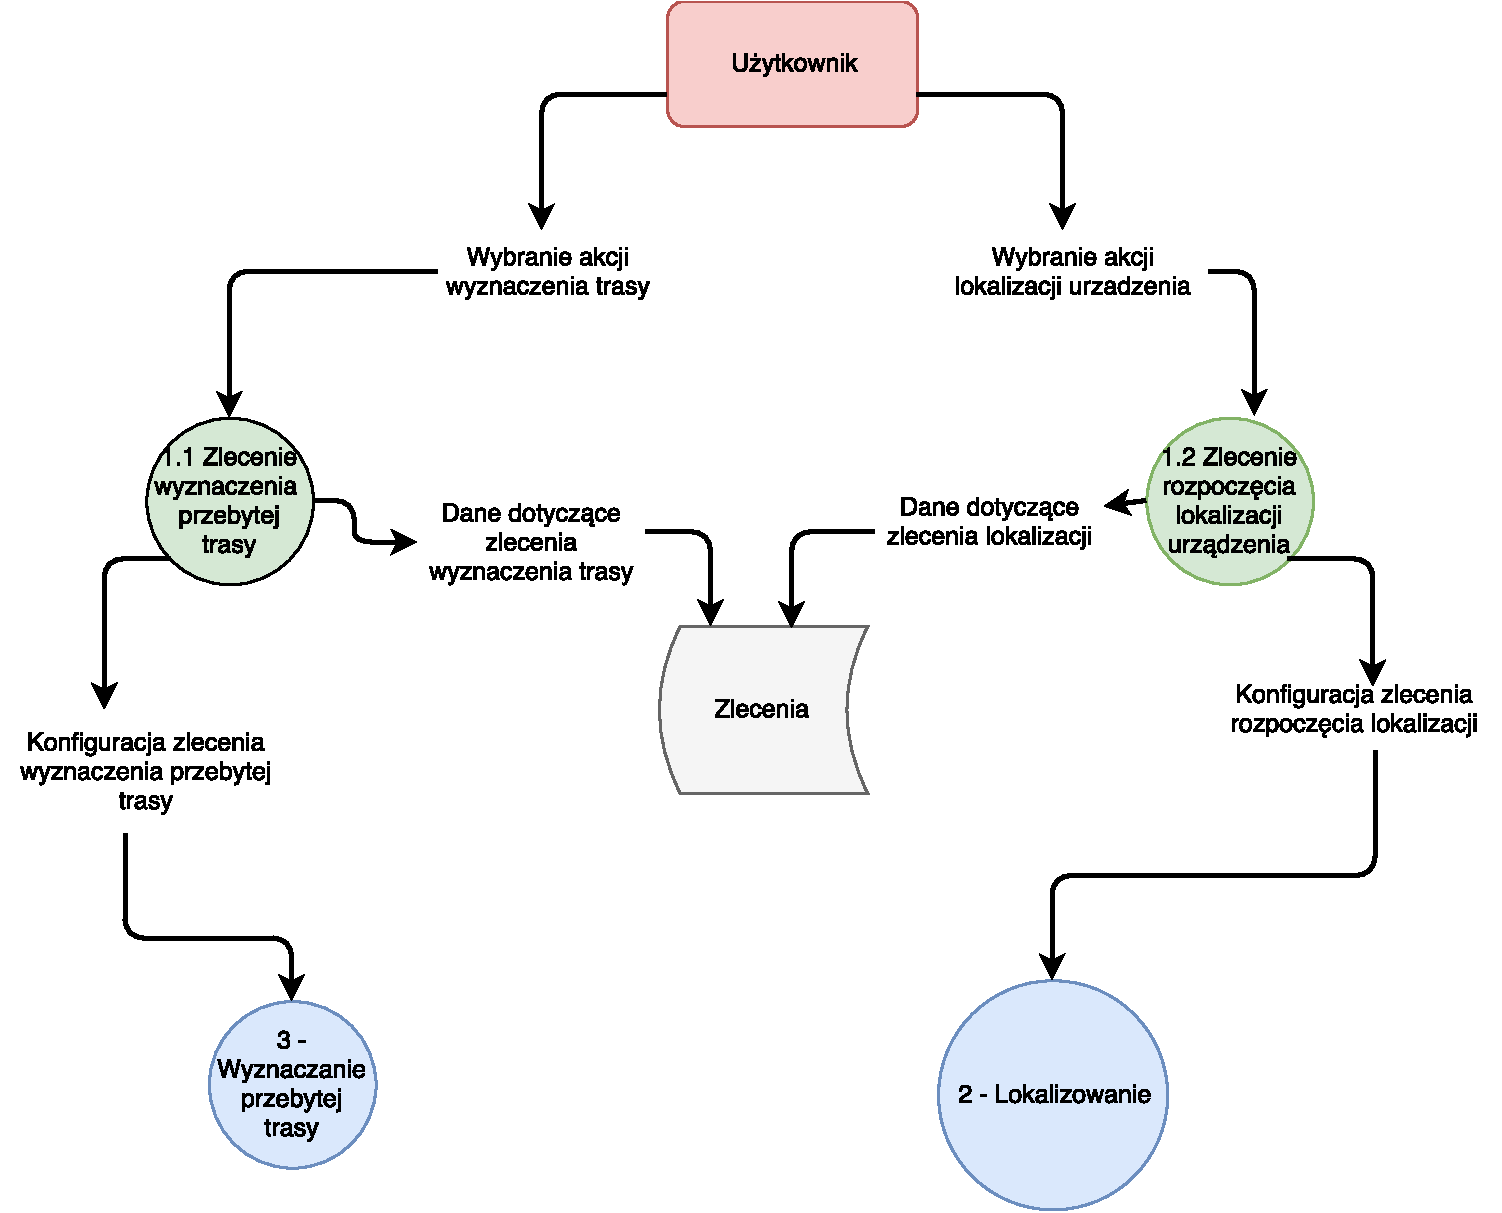
\includegraphics[scale=0.7]{DFD1.pdf}
	\end{center}
	\subsection{DFD poziom 1 - Lokalizowanie}
	\begin{center}
		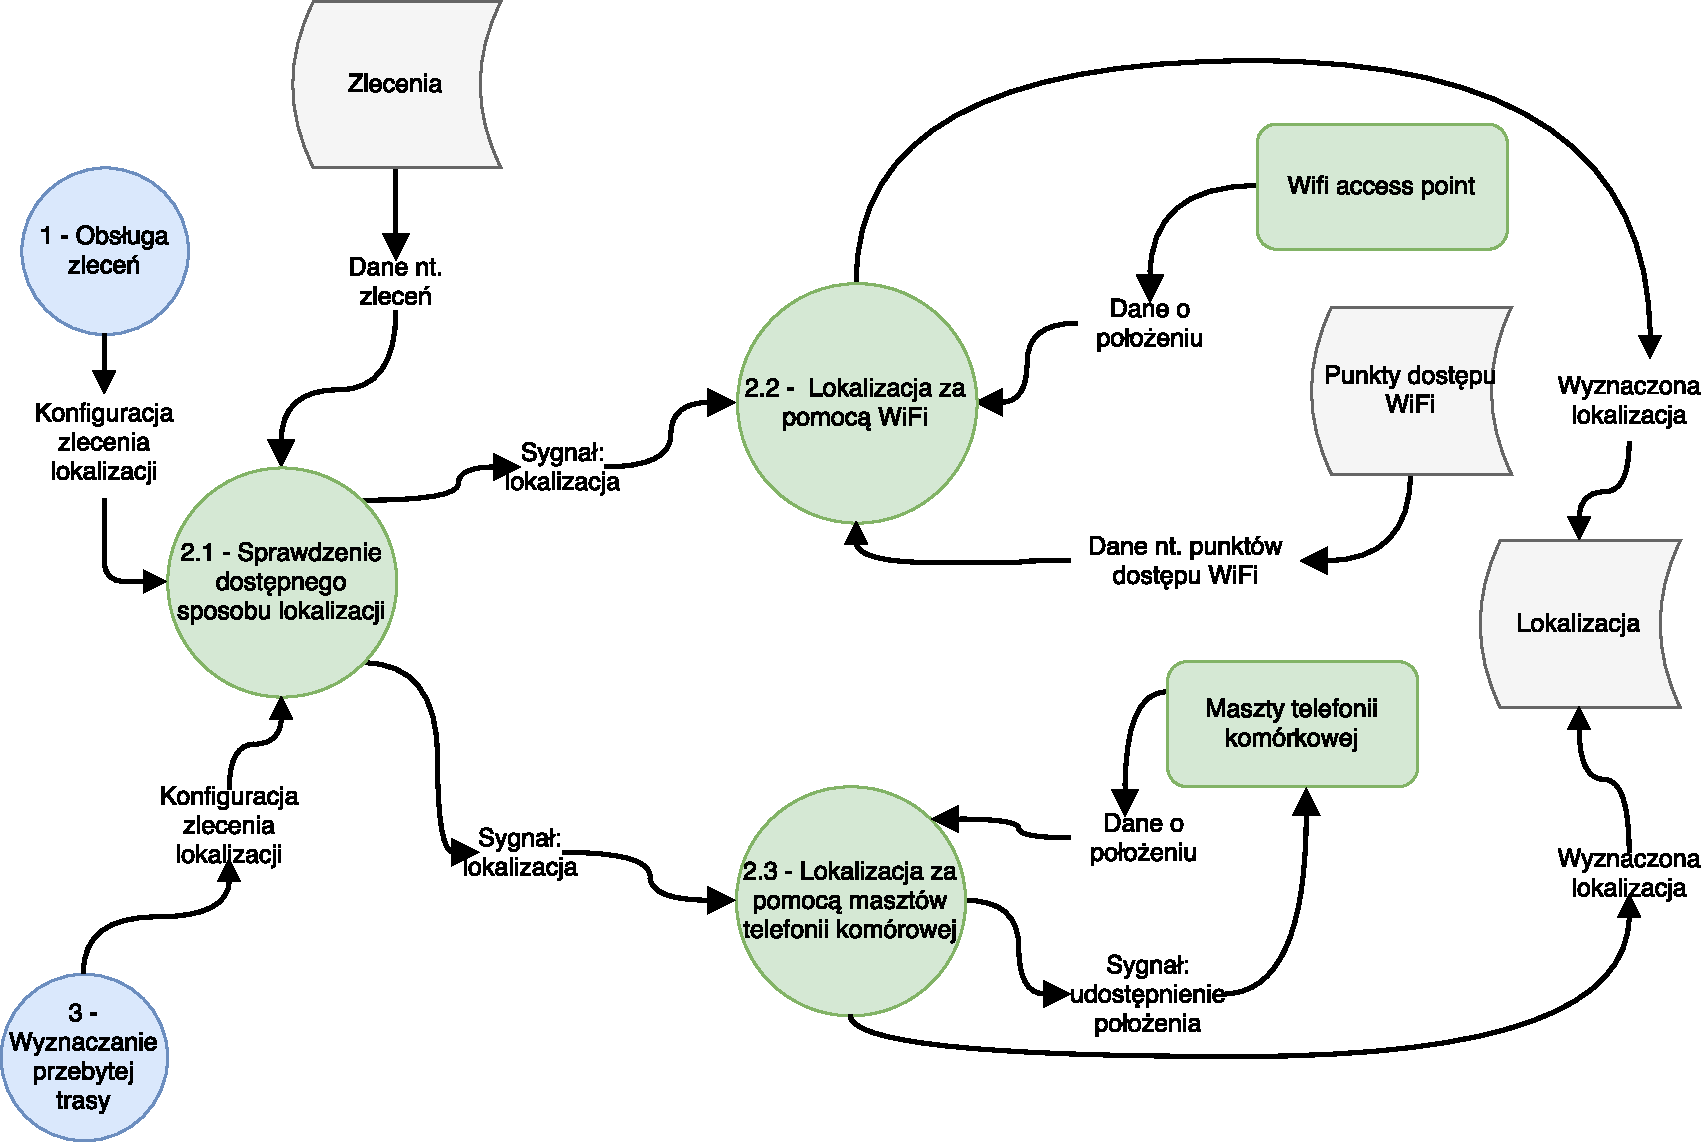
\includegraphics[scale=0.6]{DFD2.pdf}
	\end{center}
	\newpage
	\subsection{DFD poziom 1 - Wyznaczanie przebytej trasy}
	\begin{center}
		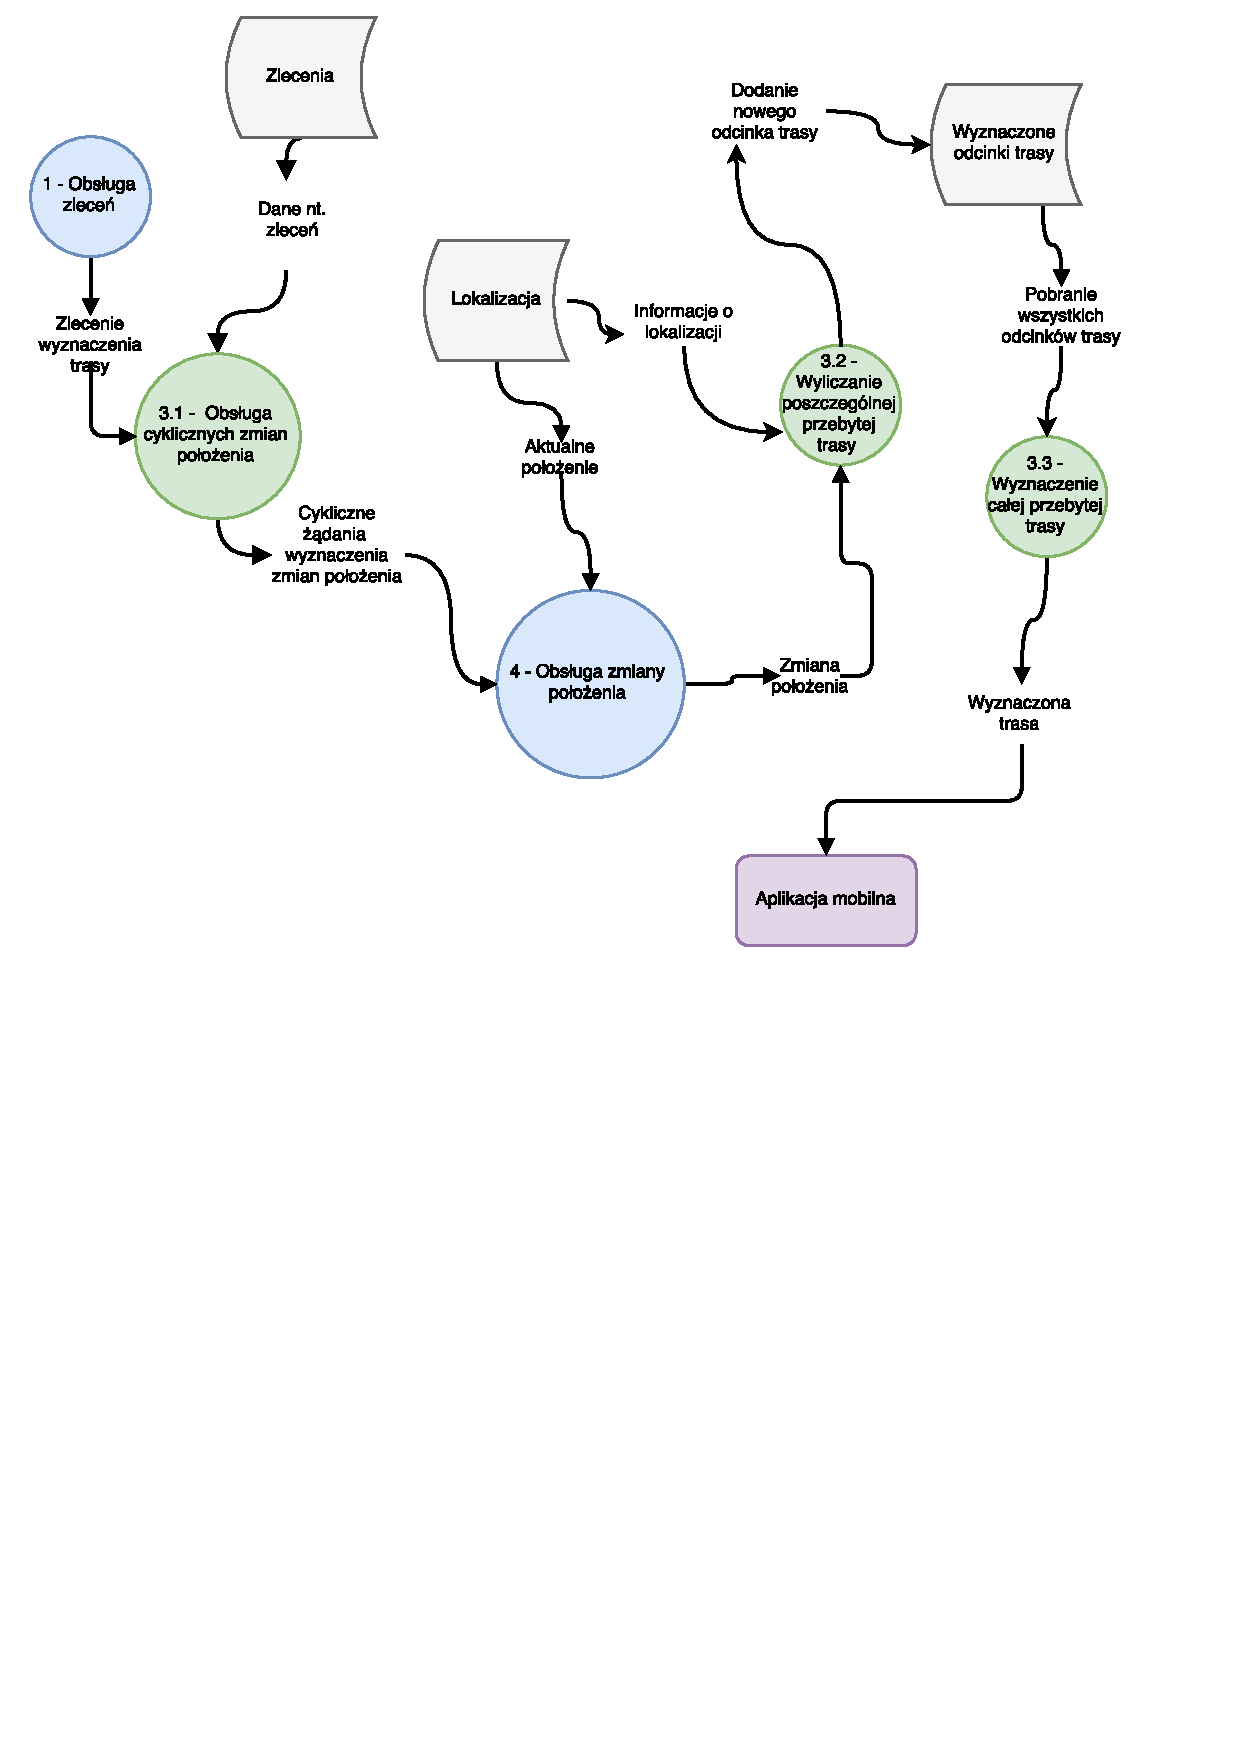
\includegraphics[scale=0.6]{DFD3.pdf}
	\end{center}
	\subsection{DFD poziom 1 - Obsługa zmiany położenia}
	\begin{center}
		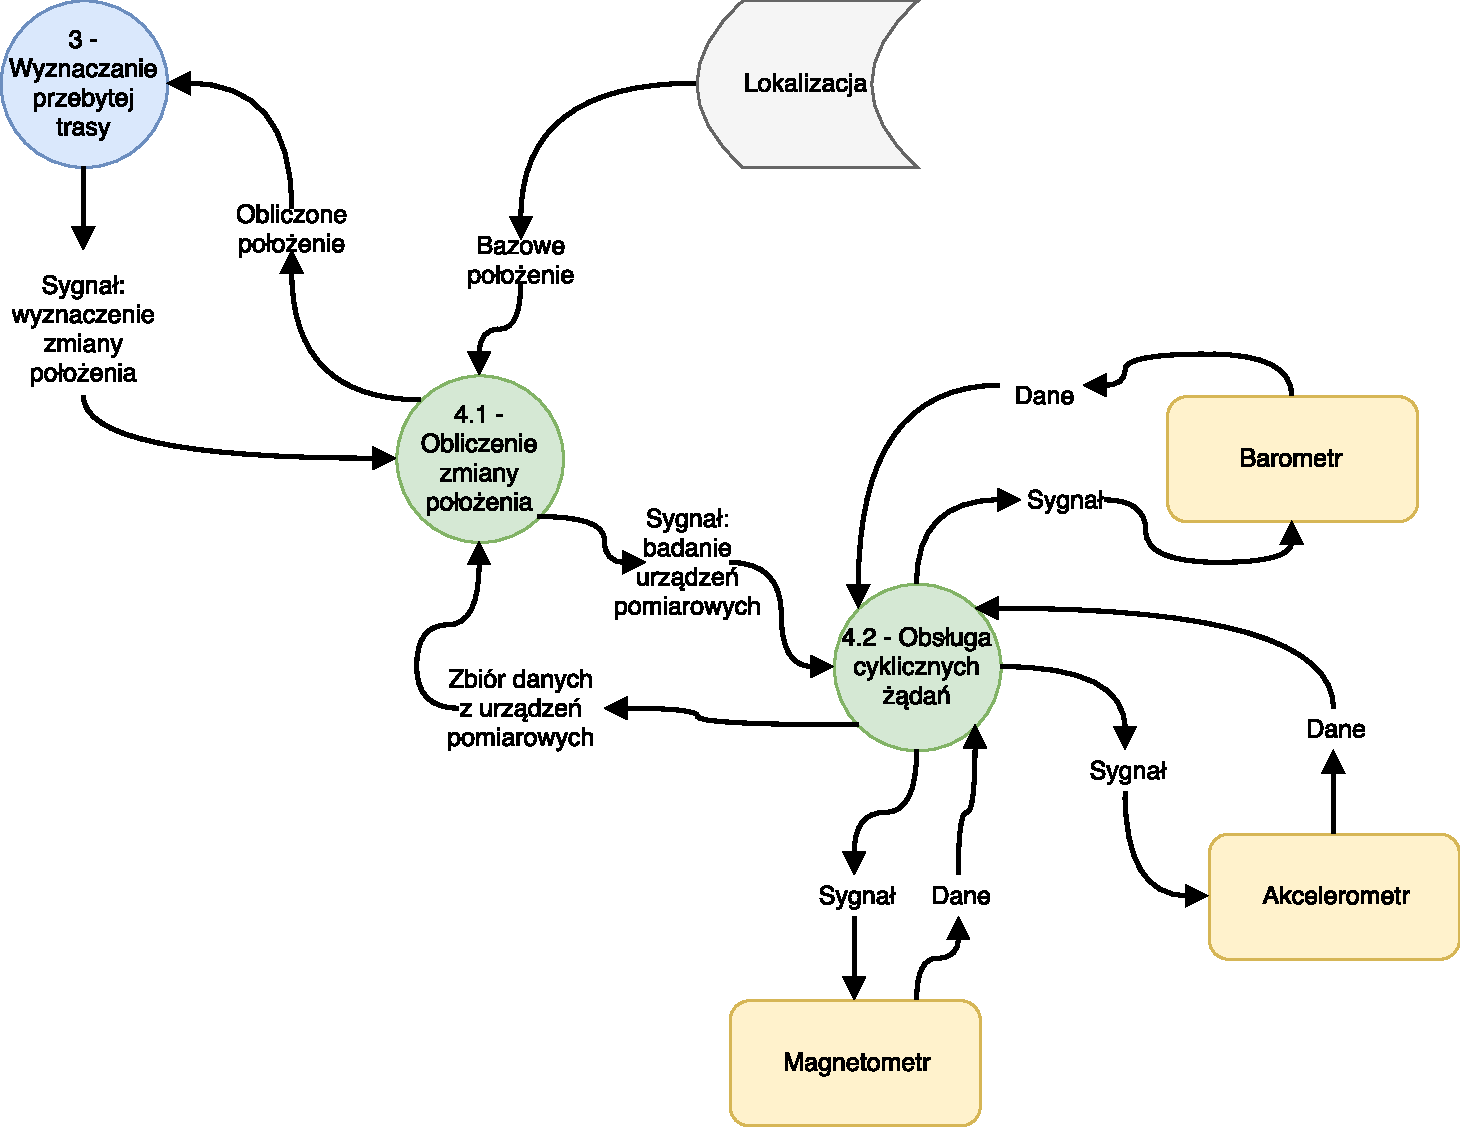
\includegraphics[scale=0.6]{DFD4.pdf}
	\end{center}
	\newpage
	\section{DFD poziom 2}
	\subsection{DFD poziom 2 }
	\begin{center}
		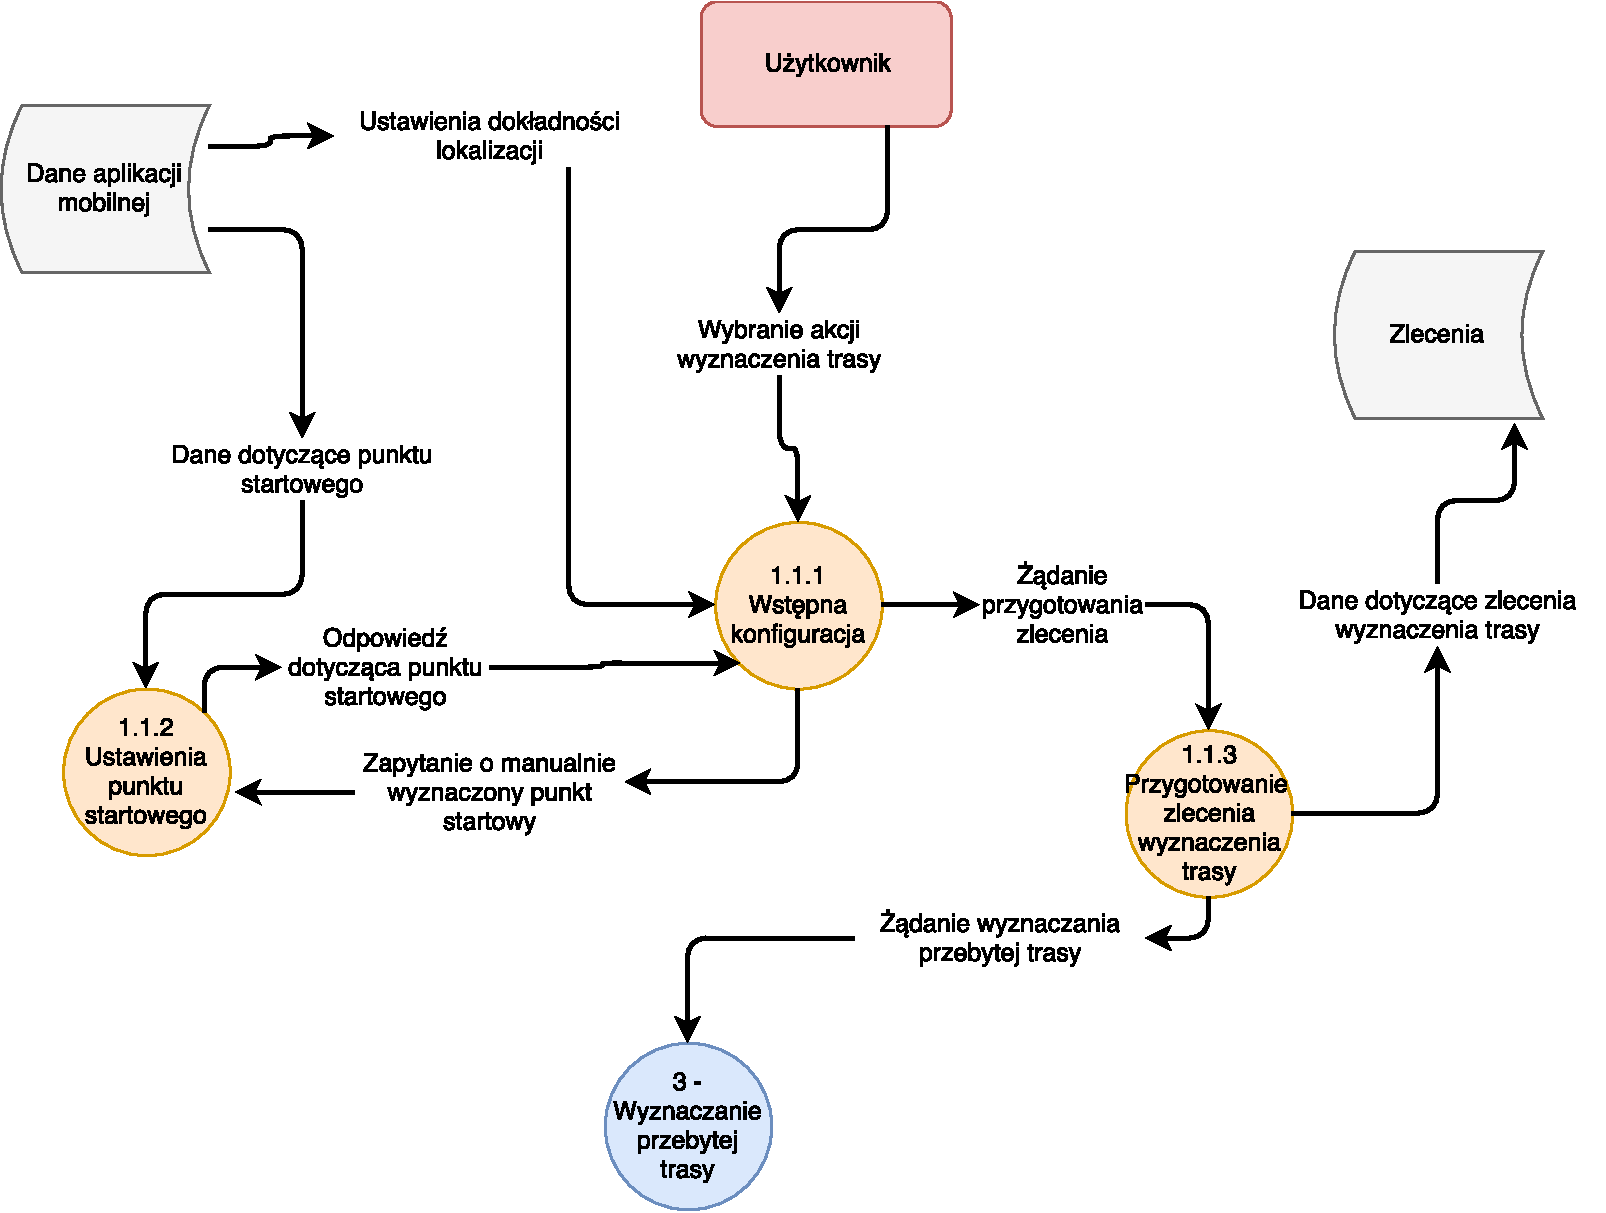
\includegraphics[scale=0.6]{DFD11.pdf}
	\end{center}
	\subsection{DFD poziom 2}
	\begin{center}
		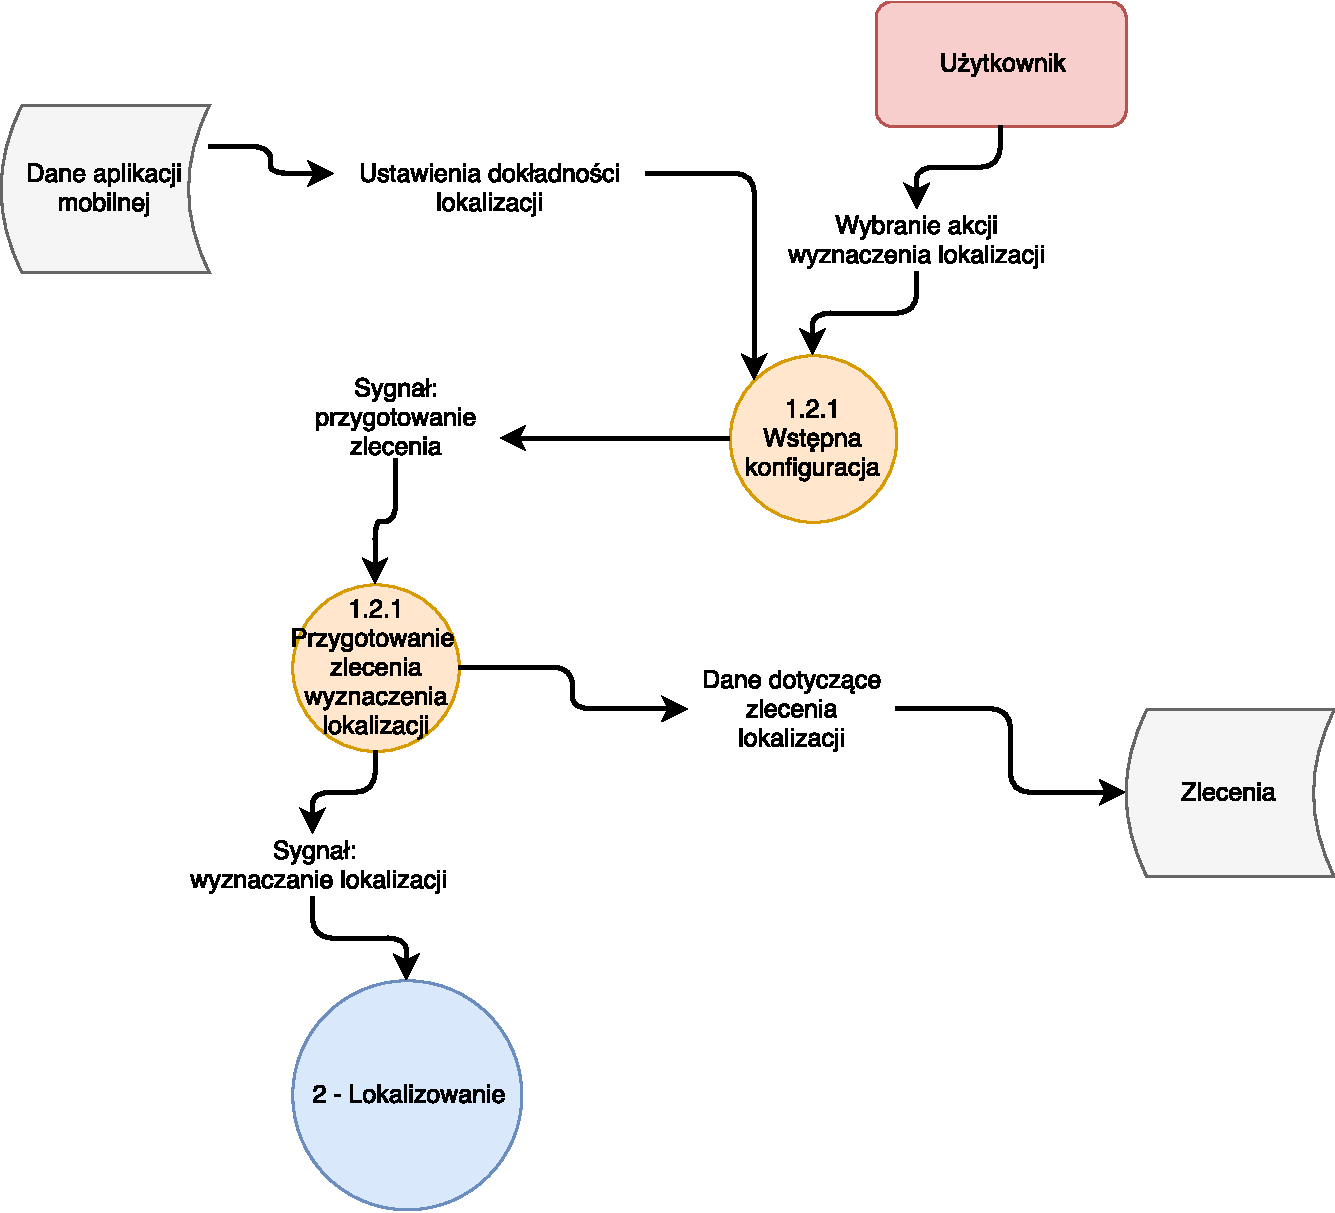
\includegraphics[scale=0.7]{DFD12.pdf}
	\end{center}
	\newpage
	\subsection{DFD poziom 2}
	\begin{center}
		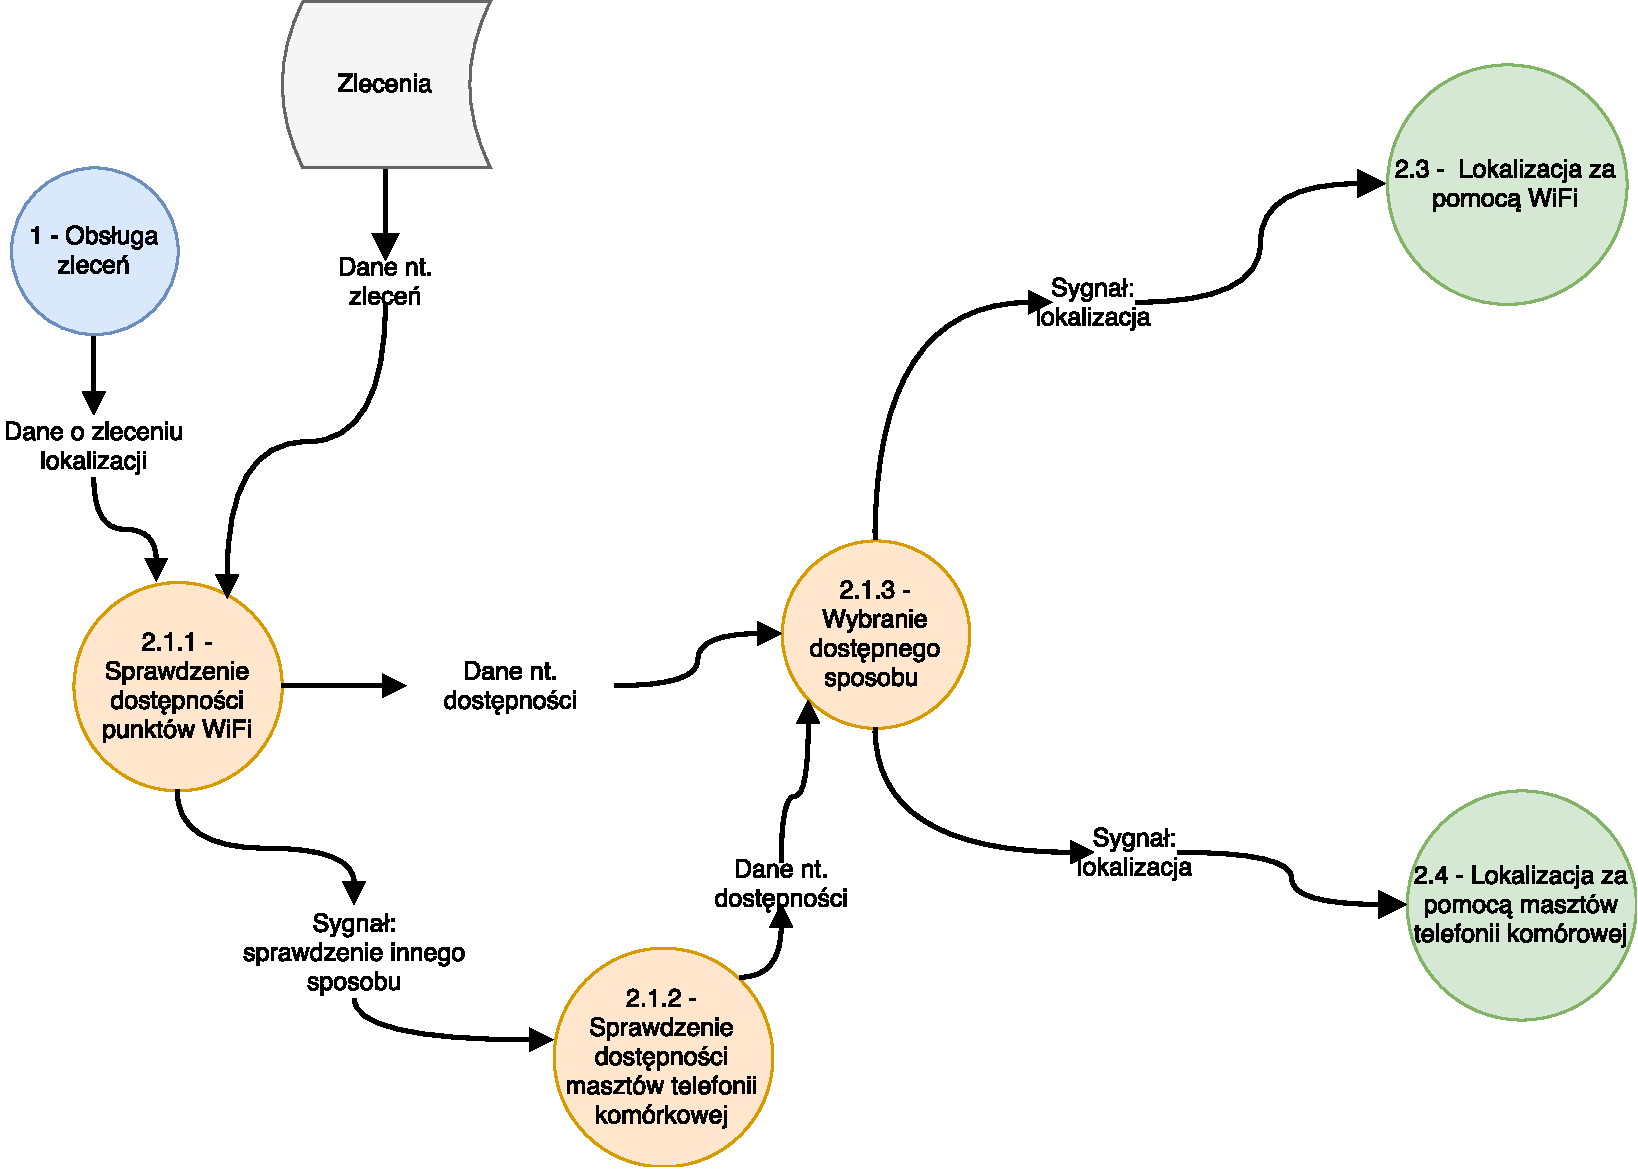
\includegraphics[scale=0.6]{DFD21.pdf}
	\end{center}
	\subsection{DFD poziom 2}
	\begin{center}
		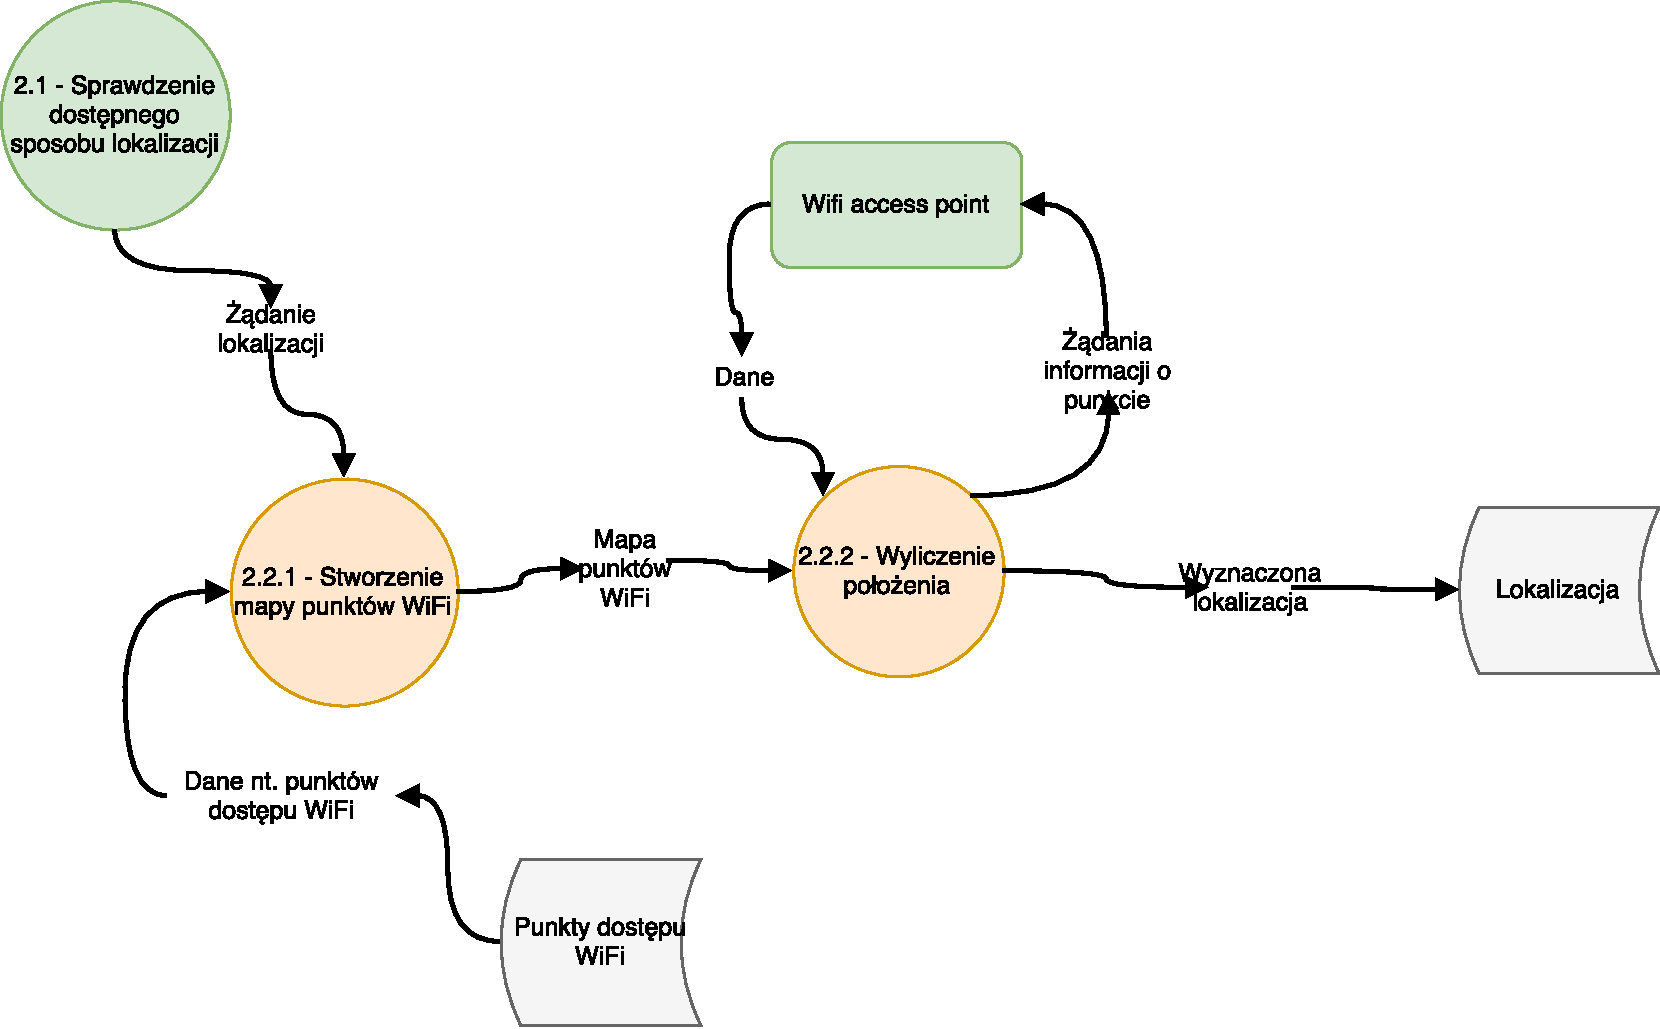
\includegraphics[scale=0.6]{DFD22.pdf}
	\end{center}
	\newpage
	\subsection{DFD poziom 2}
	\begin{center}
		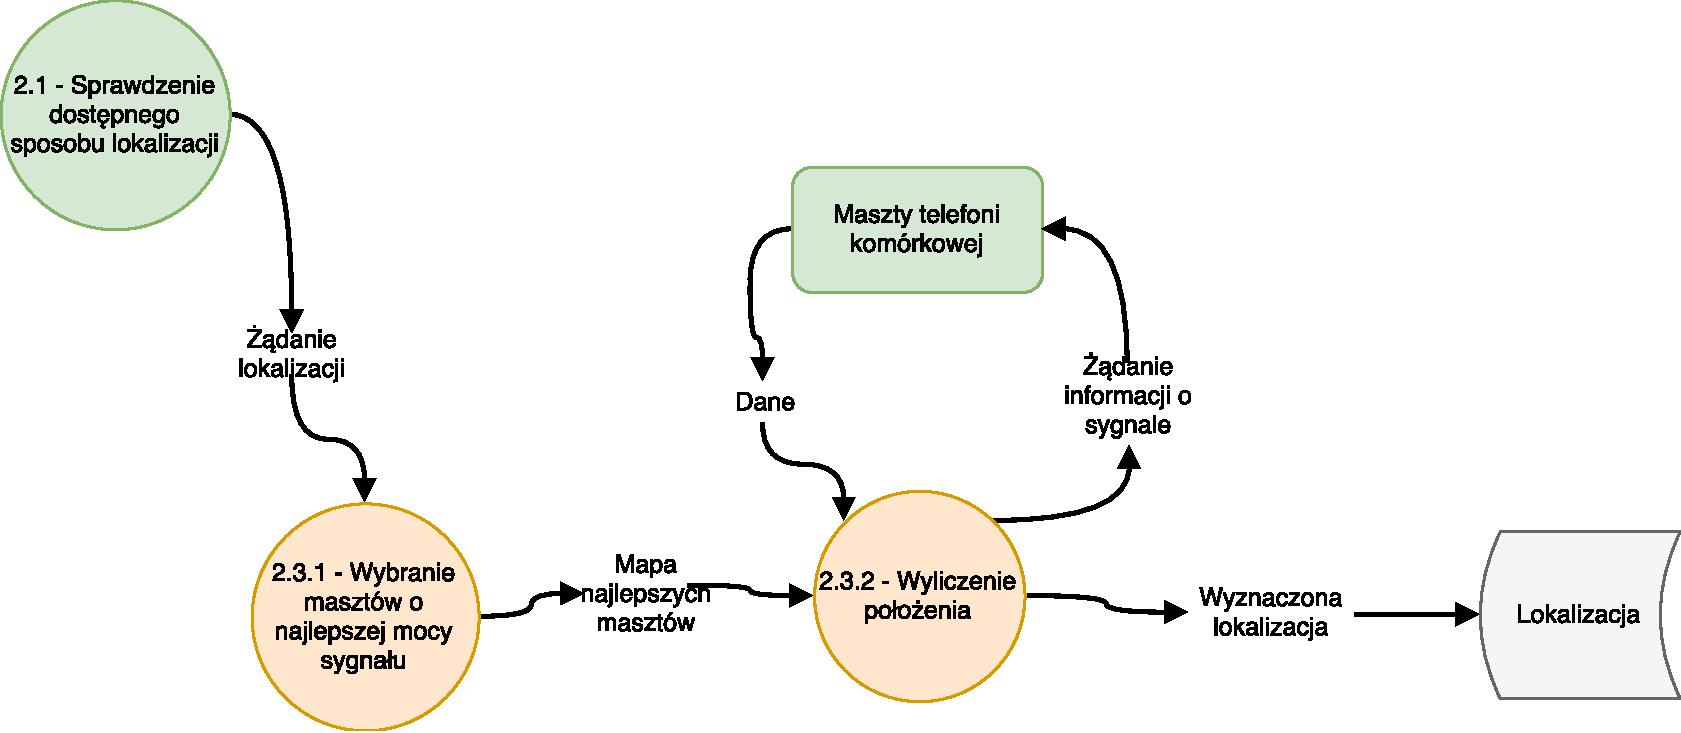
\includegraphics[scale=0.65]{DFD23.pdf}
	\end{center}
	\subsection{DFD poziom 2}
	\begin{center}
		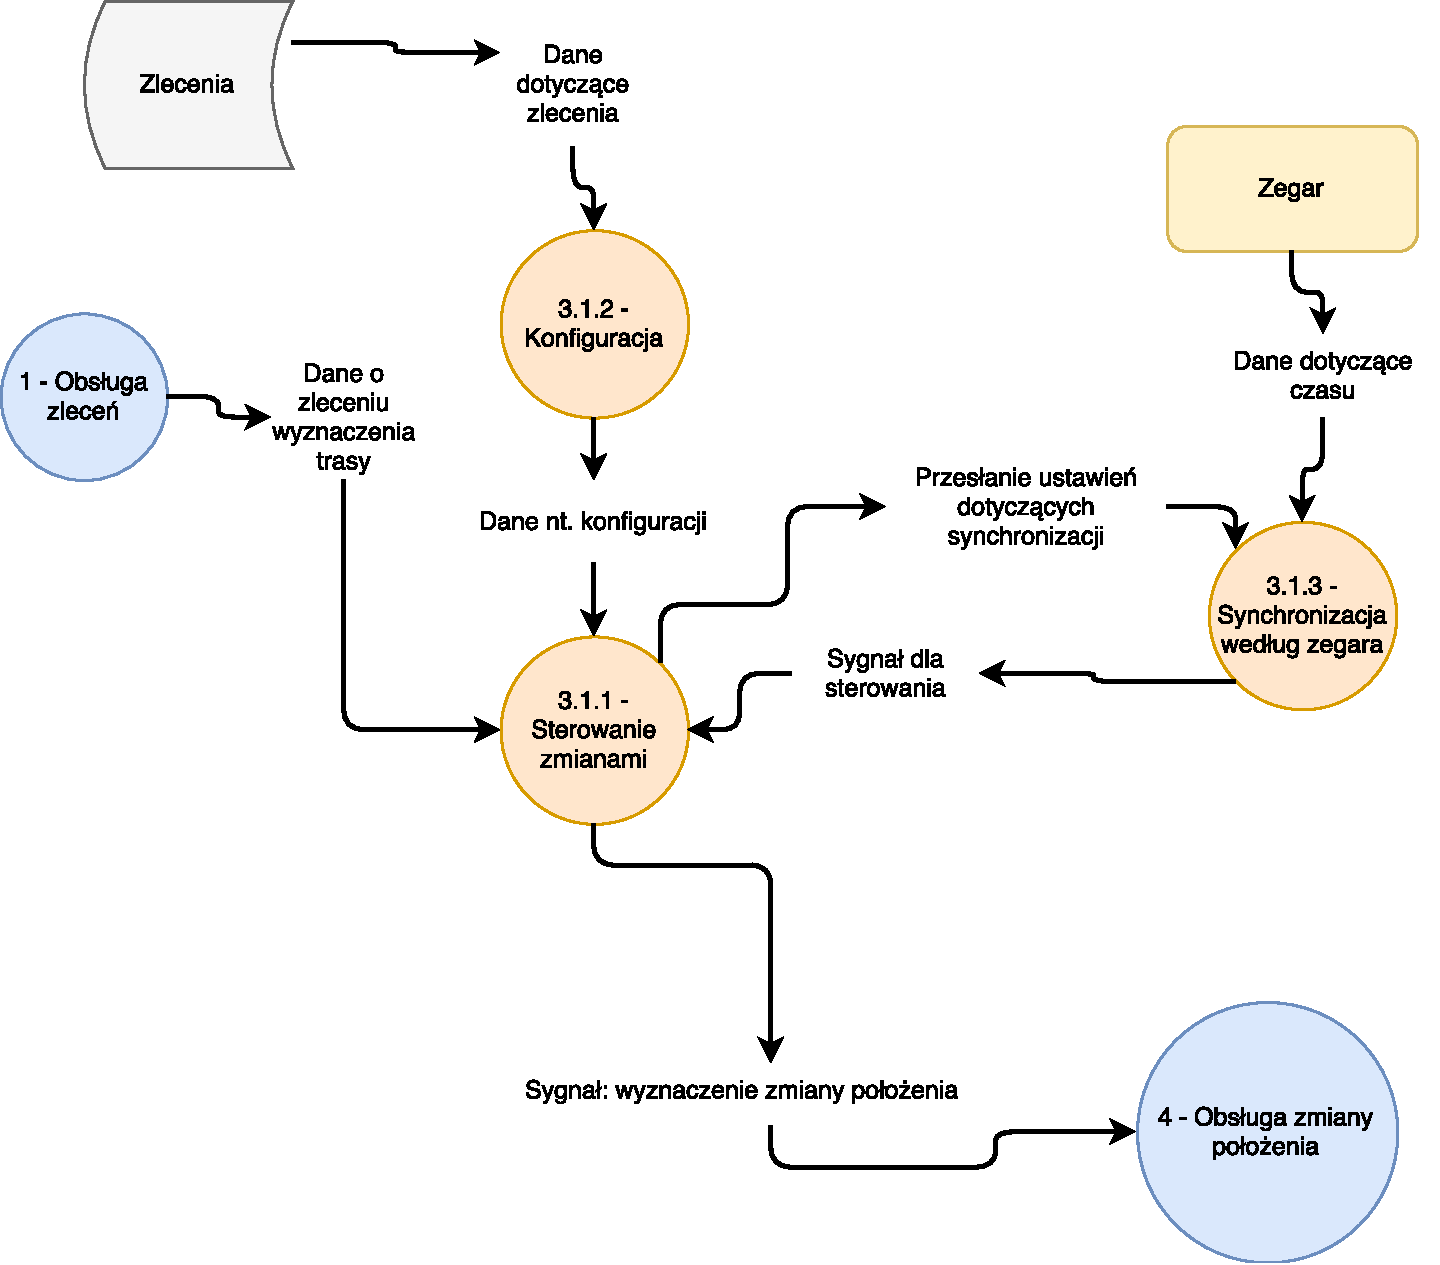
\includegraphics[scale=0.65]{DFD31.pdf}
	\end{center}
	\newpage
	\subsection{DFD poziom 2}
	\begin{center}
		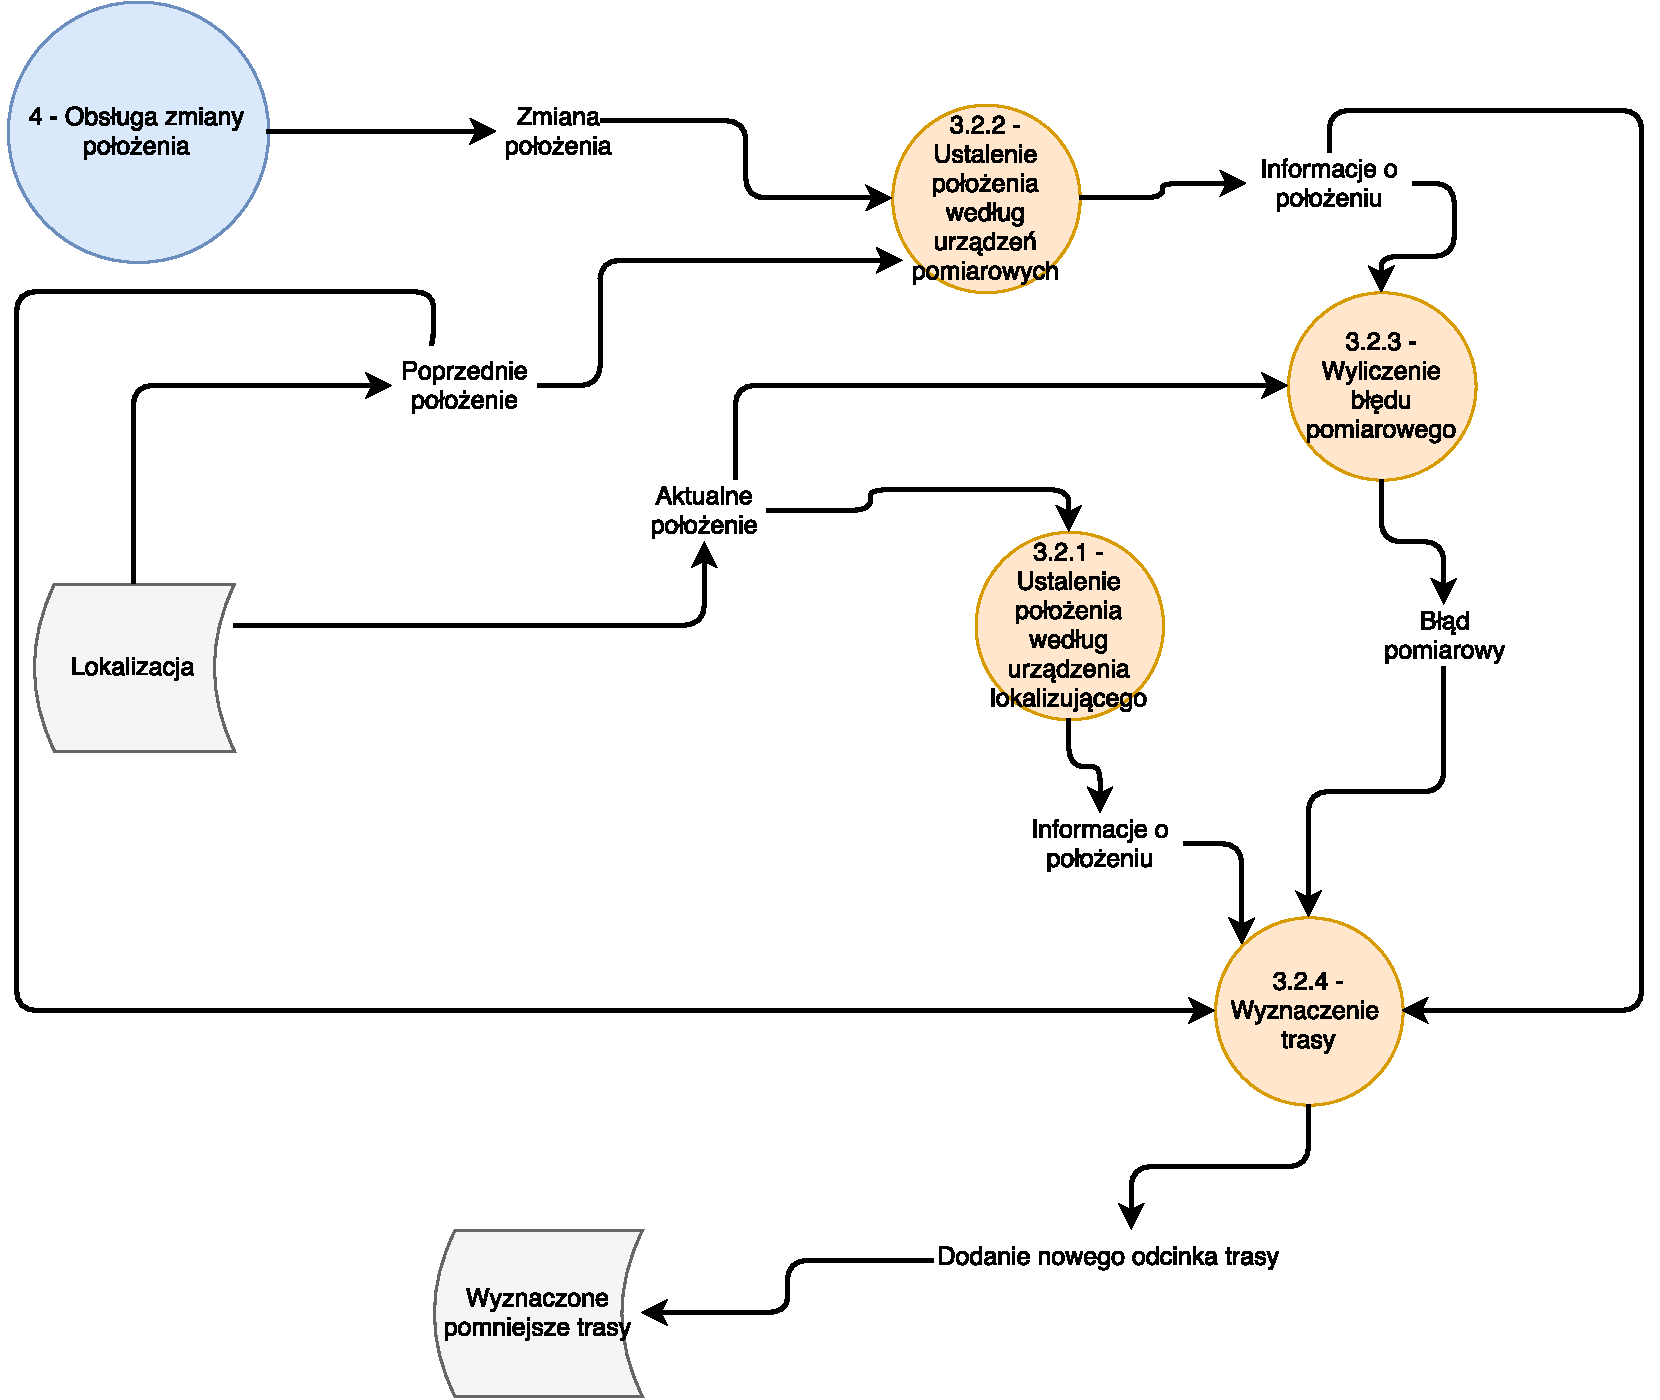
\includegraphics[scale=0.65]{DFD32.pdf}
	\end{center}
	\subsection{DFD poziom 2}
	\begin{center}
		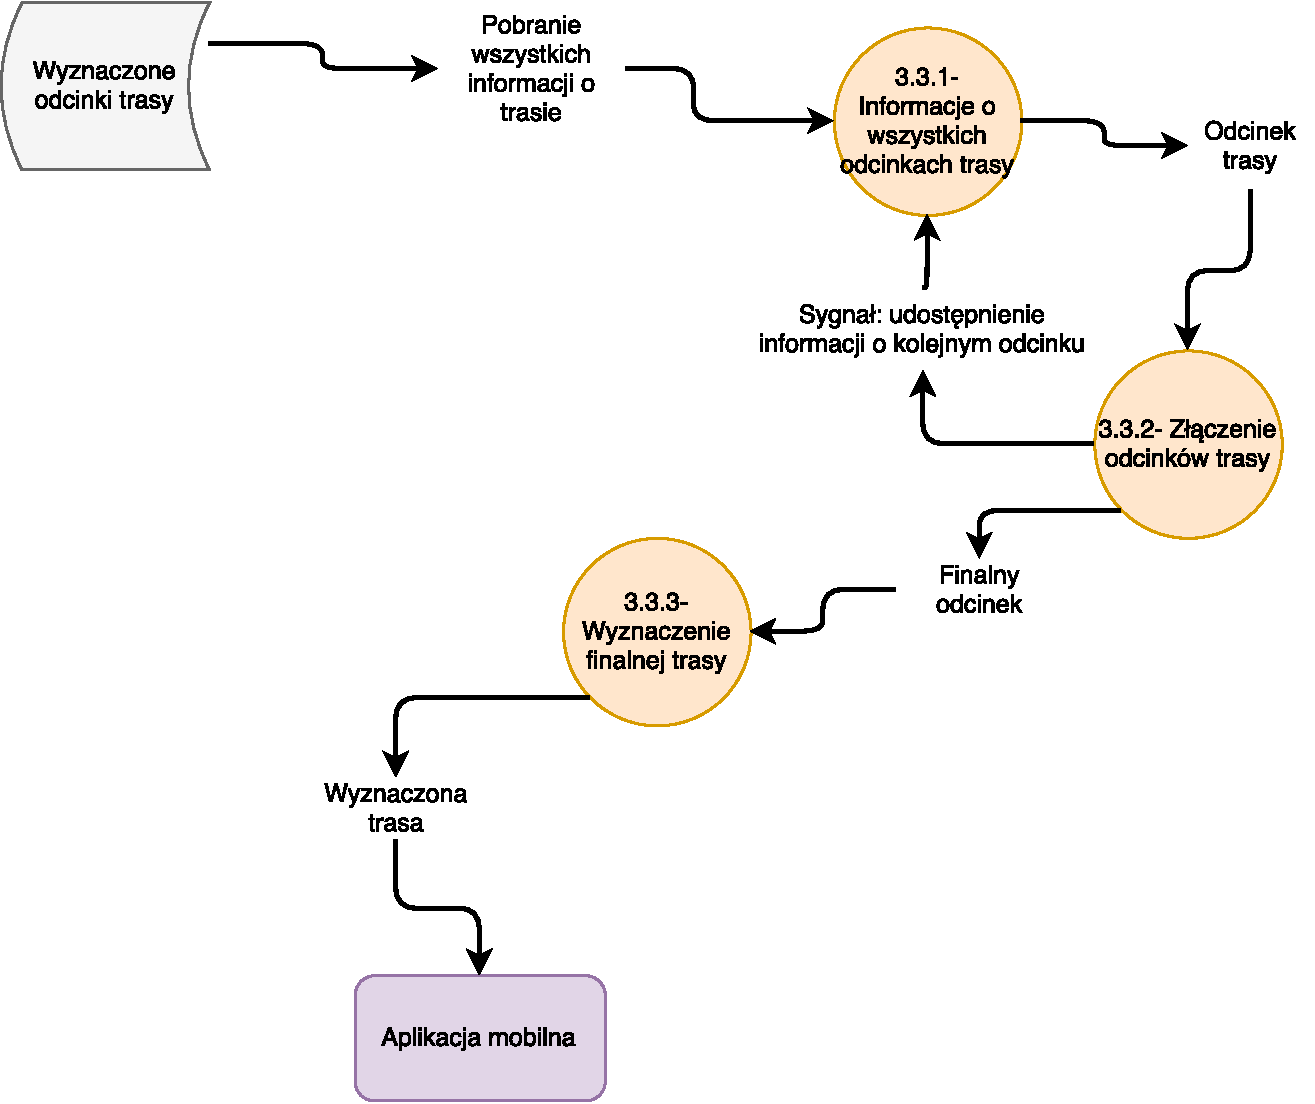
\includegraphics[scale=0.6]{DFD33.pdf}
	\end{center}
	\newpage
	\subsection{DFD poziom 2}
	\begin{center}
		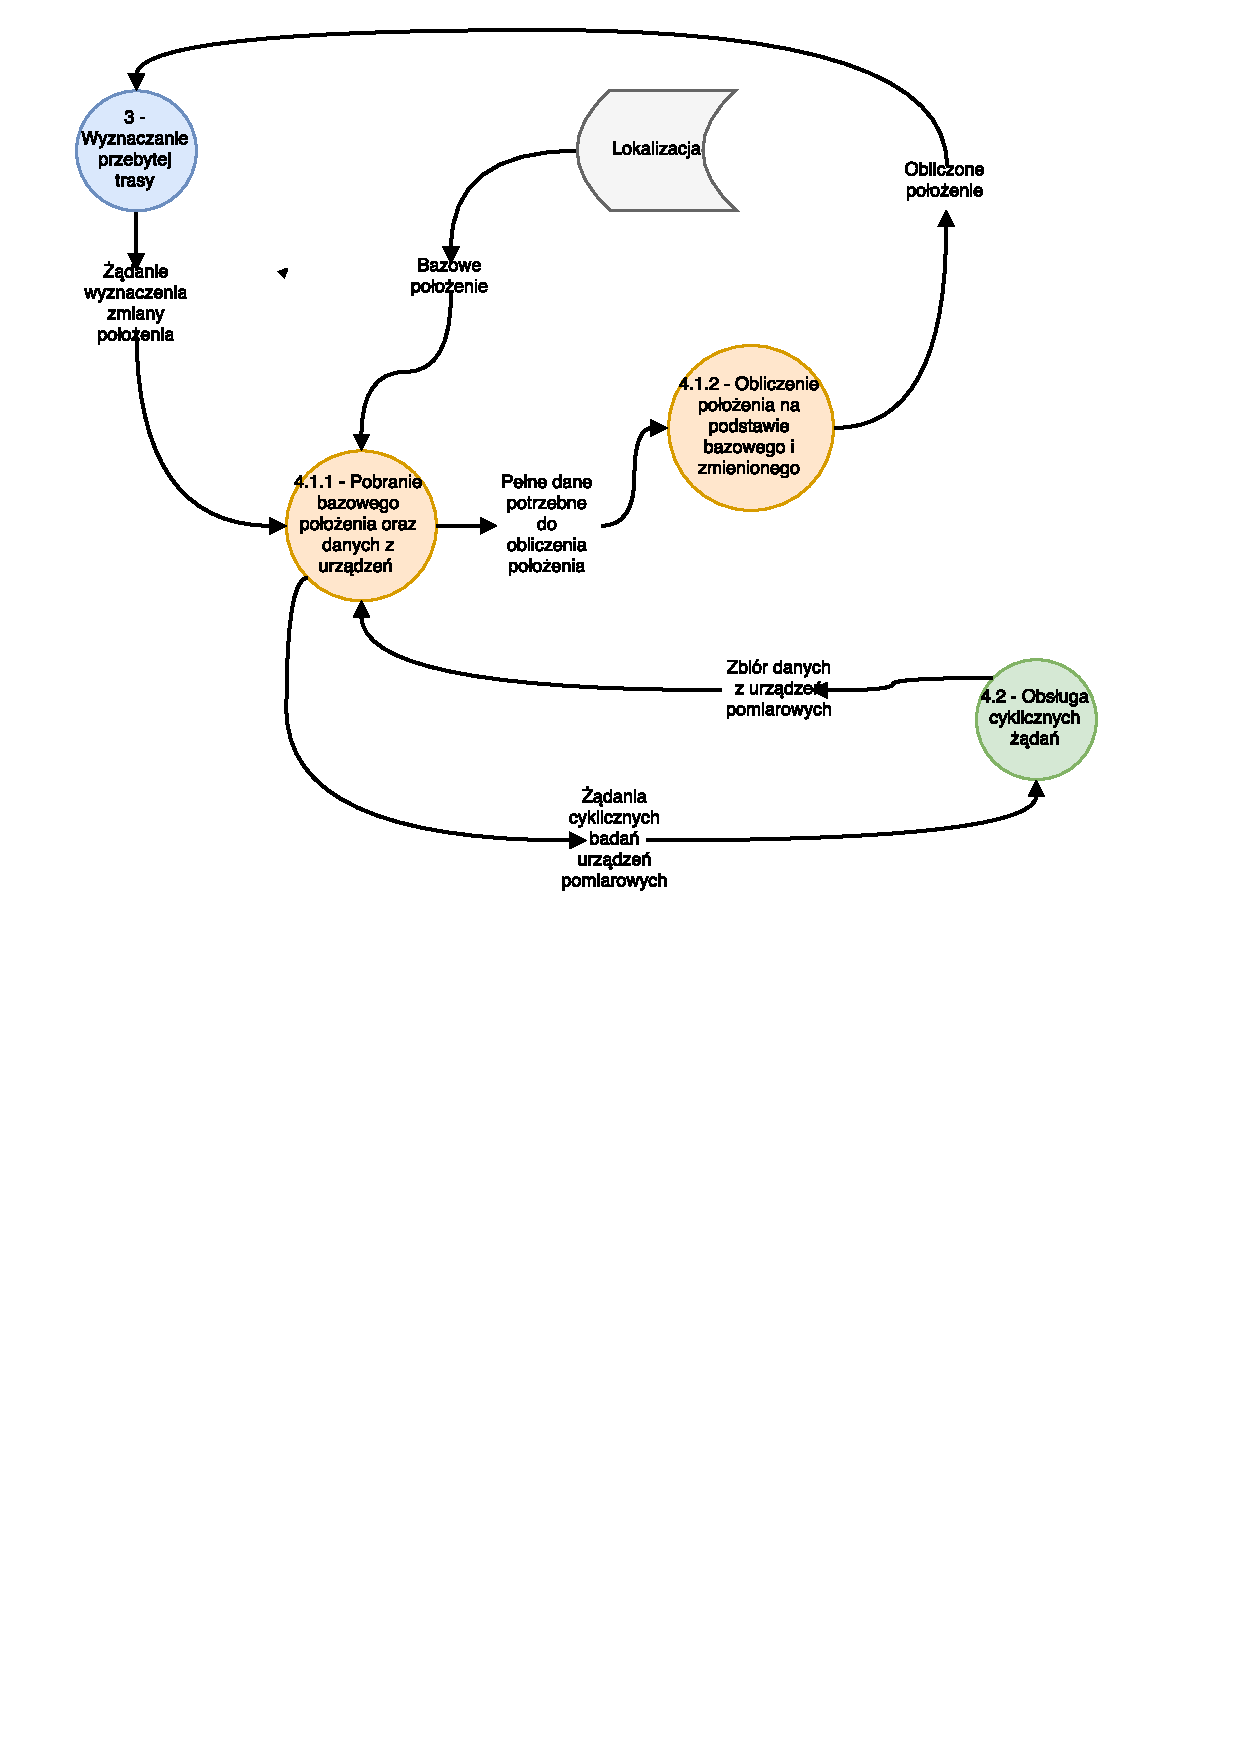
\includegraphics[scale=0.6]{DFD41.pdf}
	\end{center}
	\subsection{DFD poziom 2}
	\begin{center}
		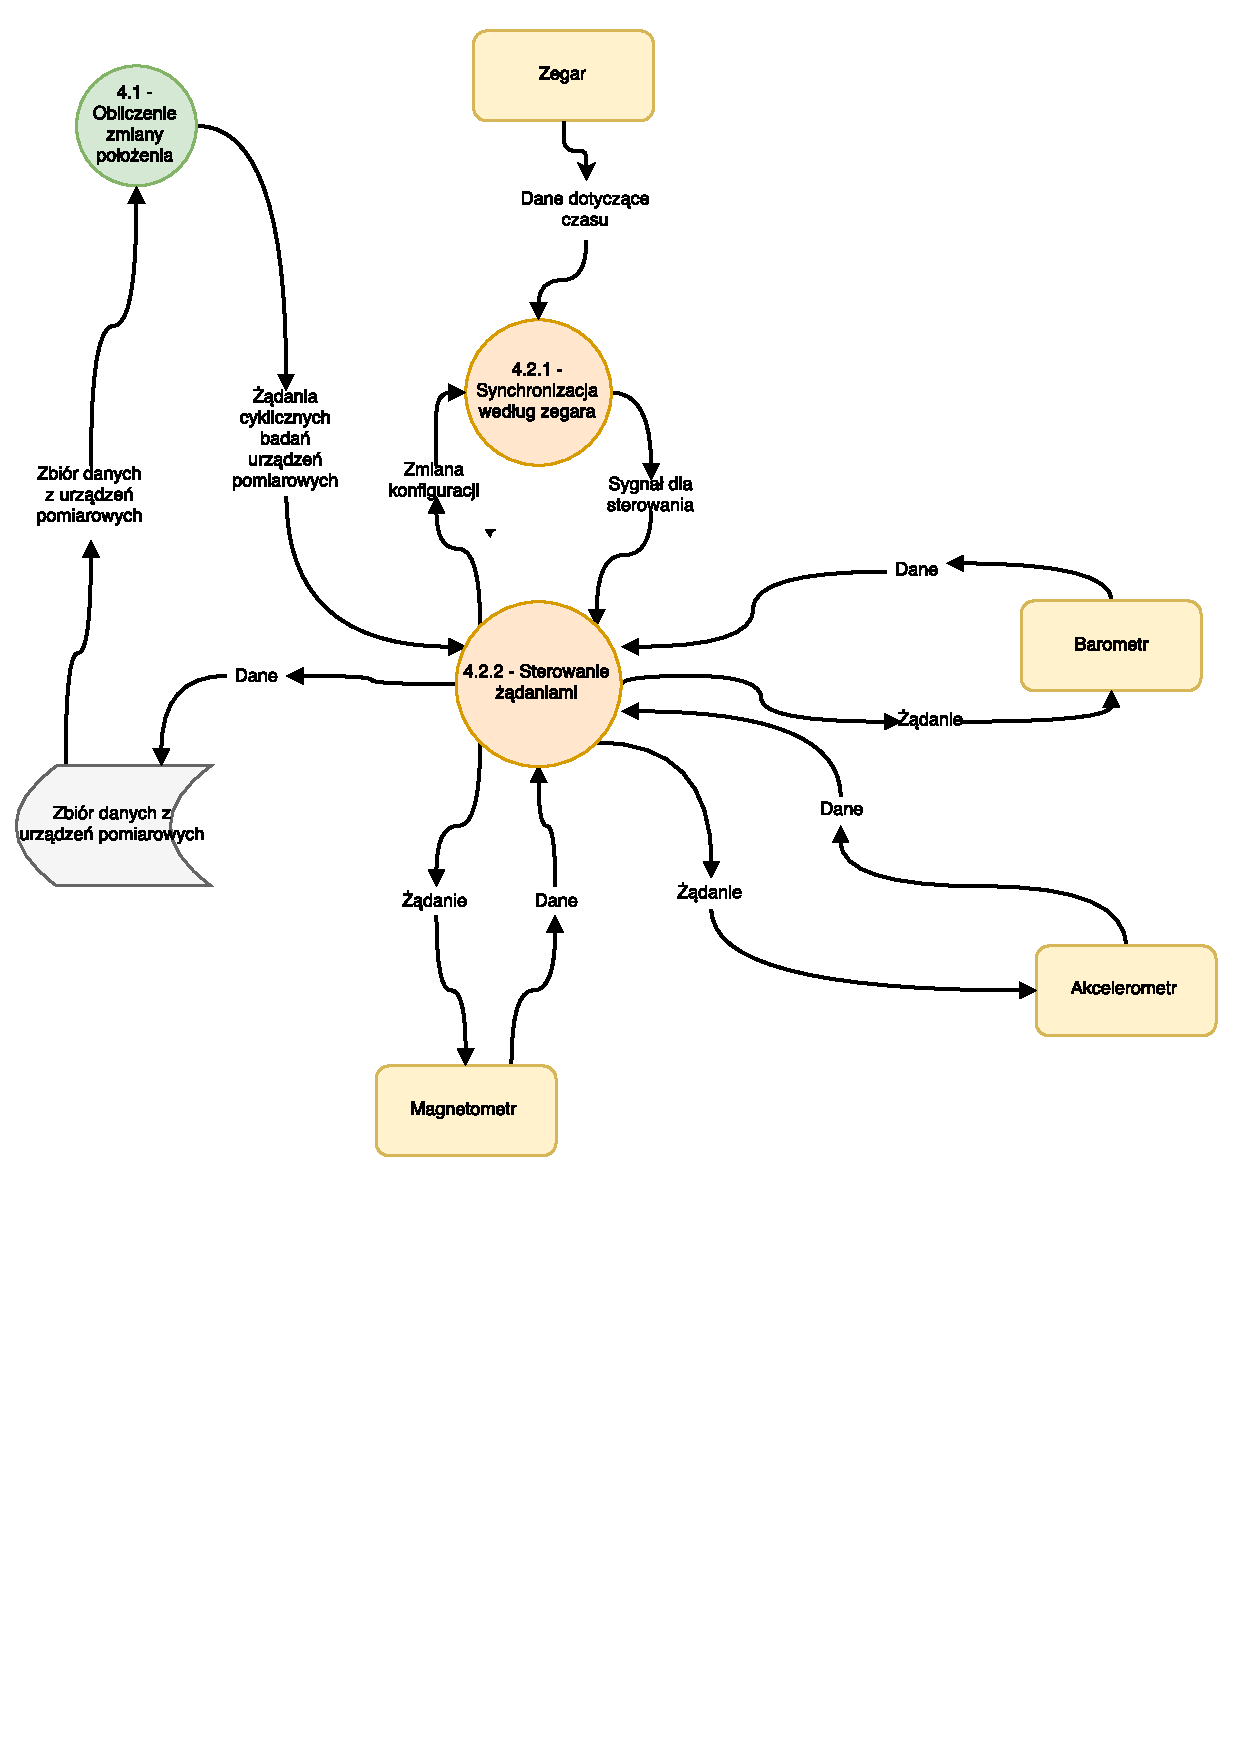
\includegraphics[scale=0.55]{DFD42.pdf}
	\end{center}
	\newpage
	\section{ERD - diagram}
	\begin{center}
		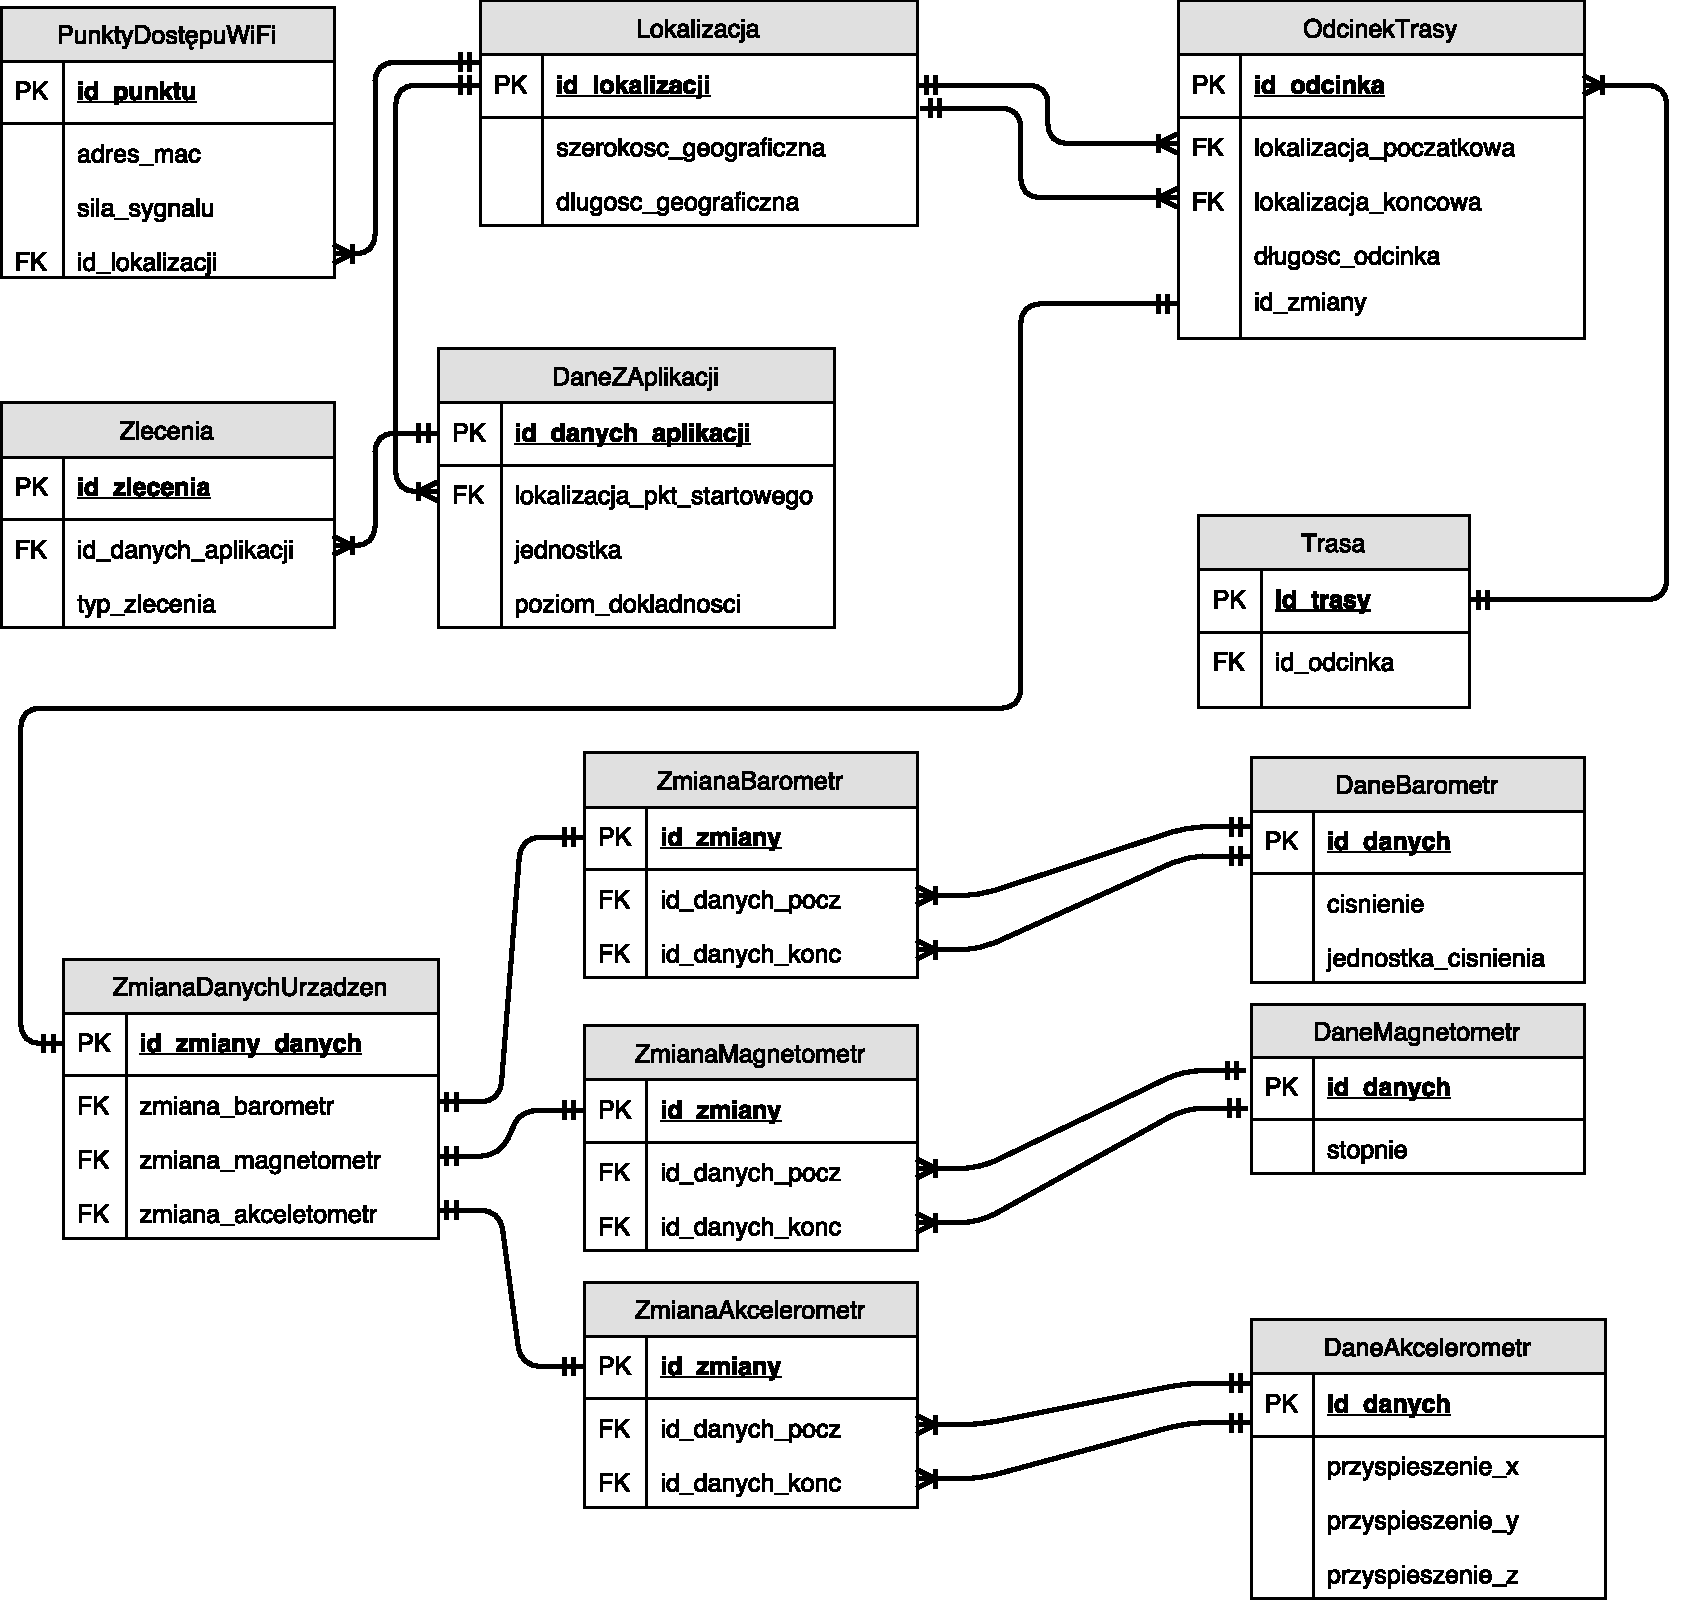
\includegraphics[scale=0.65]{ERD.pdf}
	\end{center}
	\newpage
	\section{ERD - opis}
	\subsection{PunktyDostępuWiFi}
	\begin{center}
		\includegraphics[scale=1]{punktyDostepu.PNG}
	\end{center}
	\subsection{Lokalizacja}
	\begin{center}
		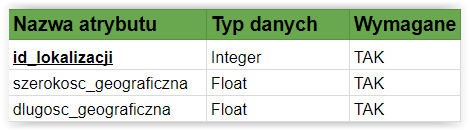
\includegraphics[scale=1]{Lokalizacja.PNG}
	\end{center}
	\subsection{Odcinek}
	\begin{center}
		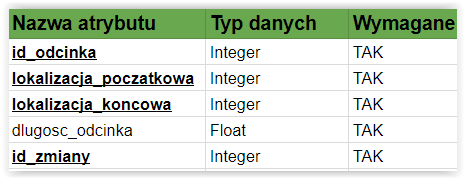
\includegraphics[scale=1]{Odcinek.PNG}
	\end{center}
	\subsection{Trasa}
	\begin{center}
		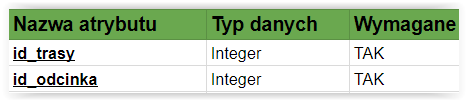
\includegraphics[scale=1]{Trasa.PNG}
	\end{center}
	\subsection{Dane z aplikacji}
	\begin{center}
		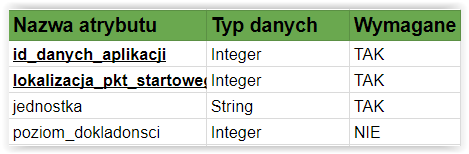
\includegraphics[scale=1]{daneAplikacji.PNG}
	\end{center}
	\subsection{Zlecenia}
	\begin{center}
		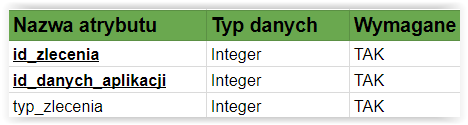
\includegraphics[scale=1]{zlecenia.PNG}
	\end{center}
	\subsection{Dane akcelerometr}
	\begin{center}
		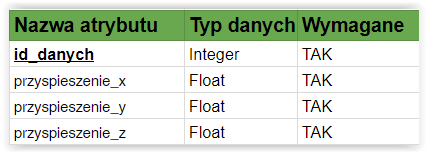
\includegraphics[scale=1]{daneAkcelerometr.PNG}
	\end{center}
	\subsection{Dane magnetometr}
	\begin{center}
		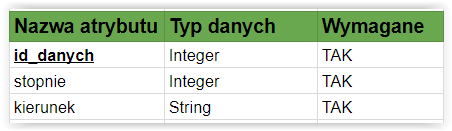
\includegraphics[scale=1]{daneMagnetometr.PNG}
	\end{center}
	\subsection{Dane barometr}
	\begin{center}
		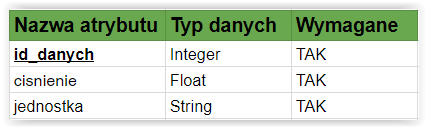
\includegraphics[scale=1]{daneBarometr.PNG}
	\end{center}
	\subsection{Dane zmiana}
	\begin{center}
		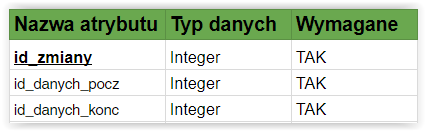
\includegraphics[scale=1]{zmianaBarometr.PNG}
	\end{center}
	\subsection{Zmiana}
	\begin{center}
		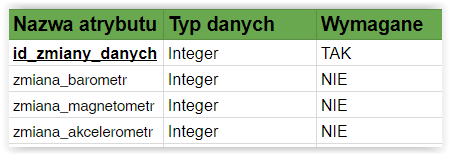
\includegraphics[scale=1]{zmianaDanych.PNG}
	\end{center}
	\newpage
	\section{STD}
	\subsection{STD poziom 0}
	\begin{center}
		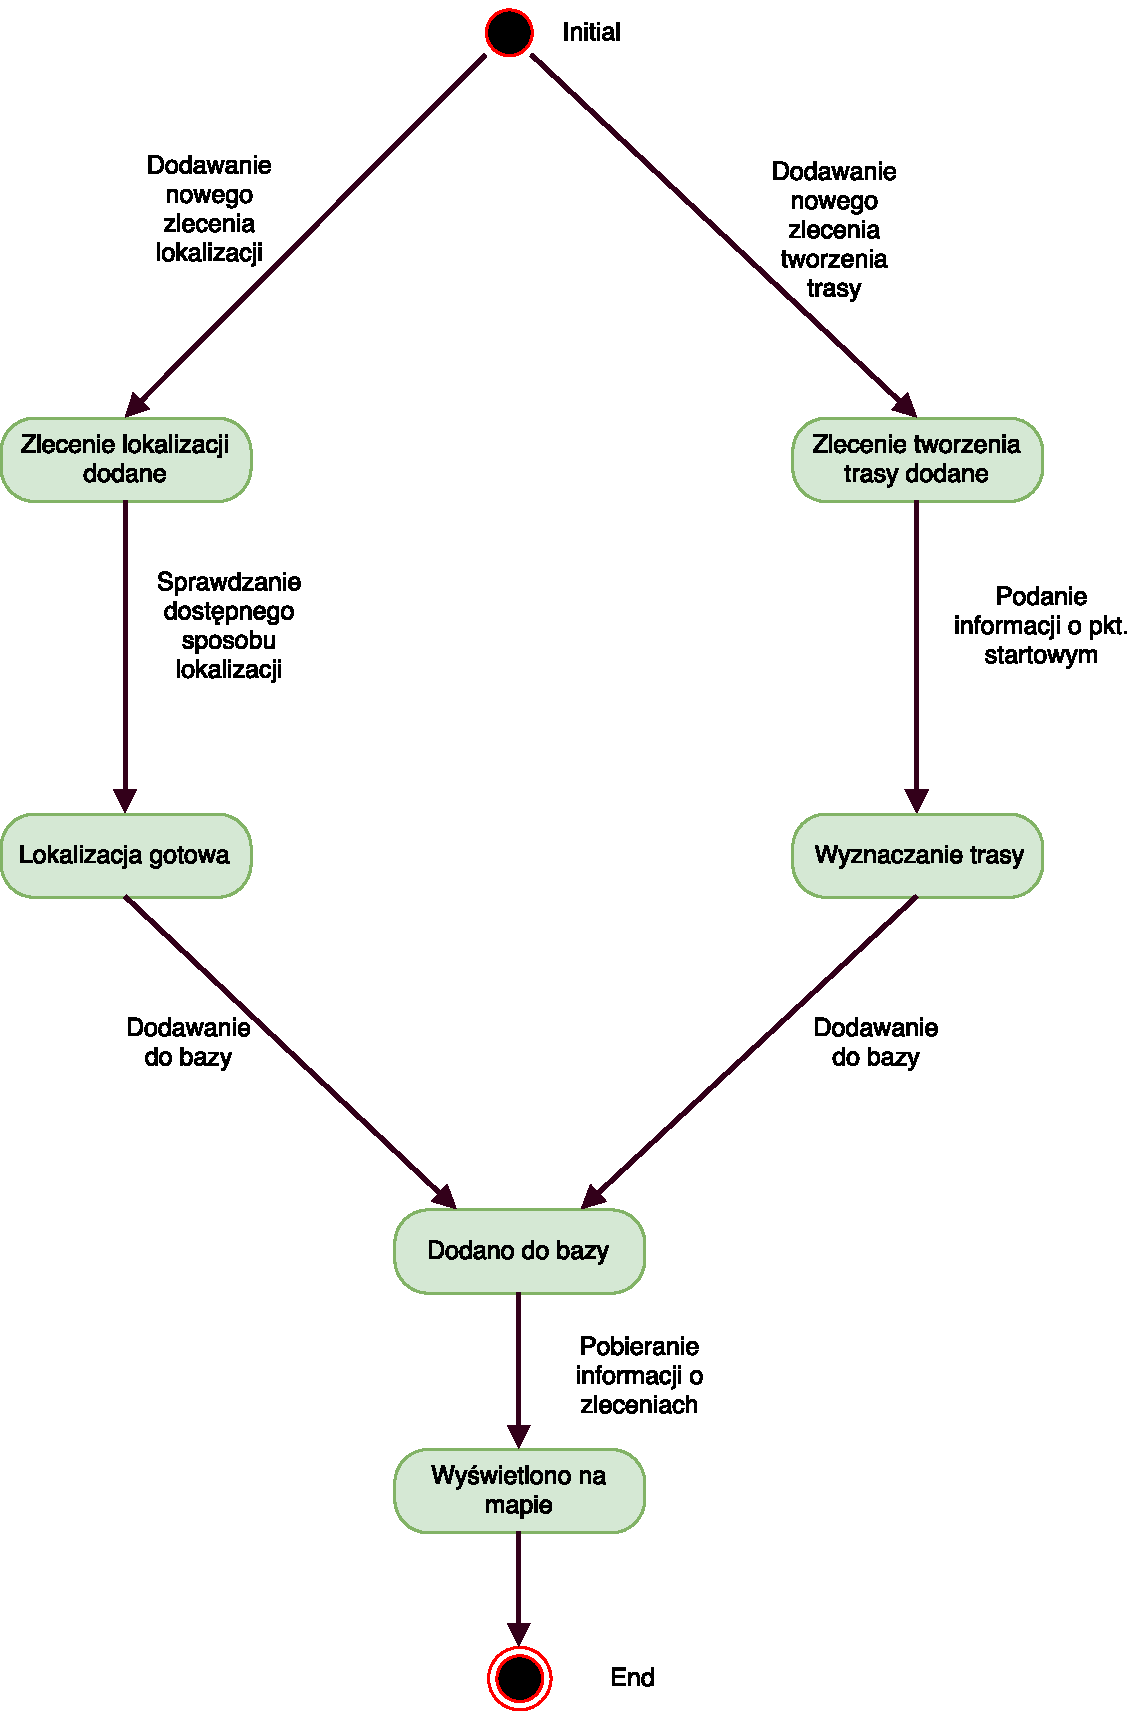
\includegraphics[scale=0.9]{STD0.pdf}
	\end{center}
	\newpage
	\subsection{STD poziom 1}
	\begin{center}
		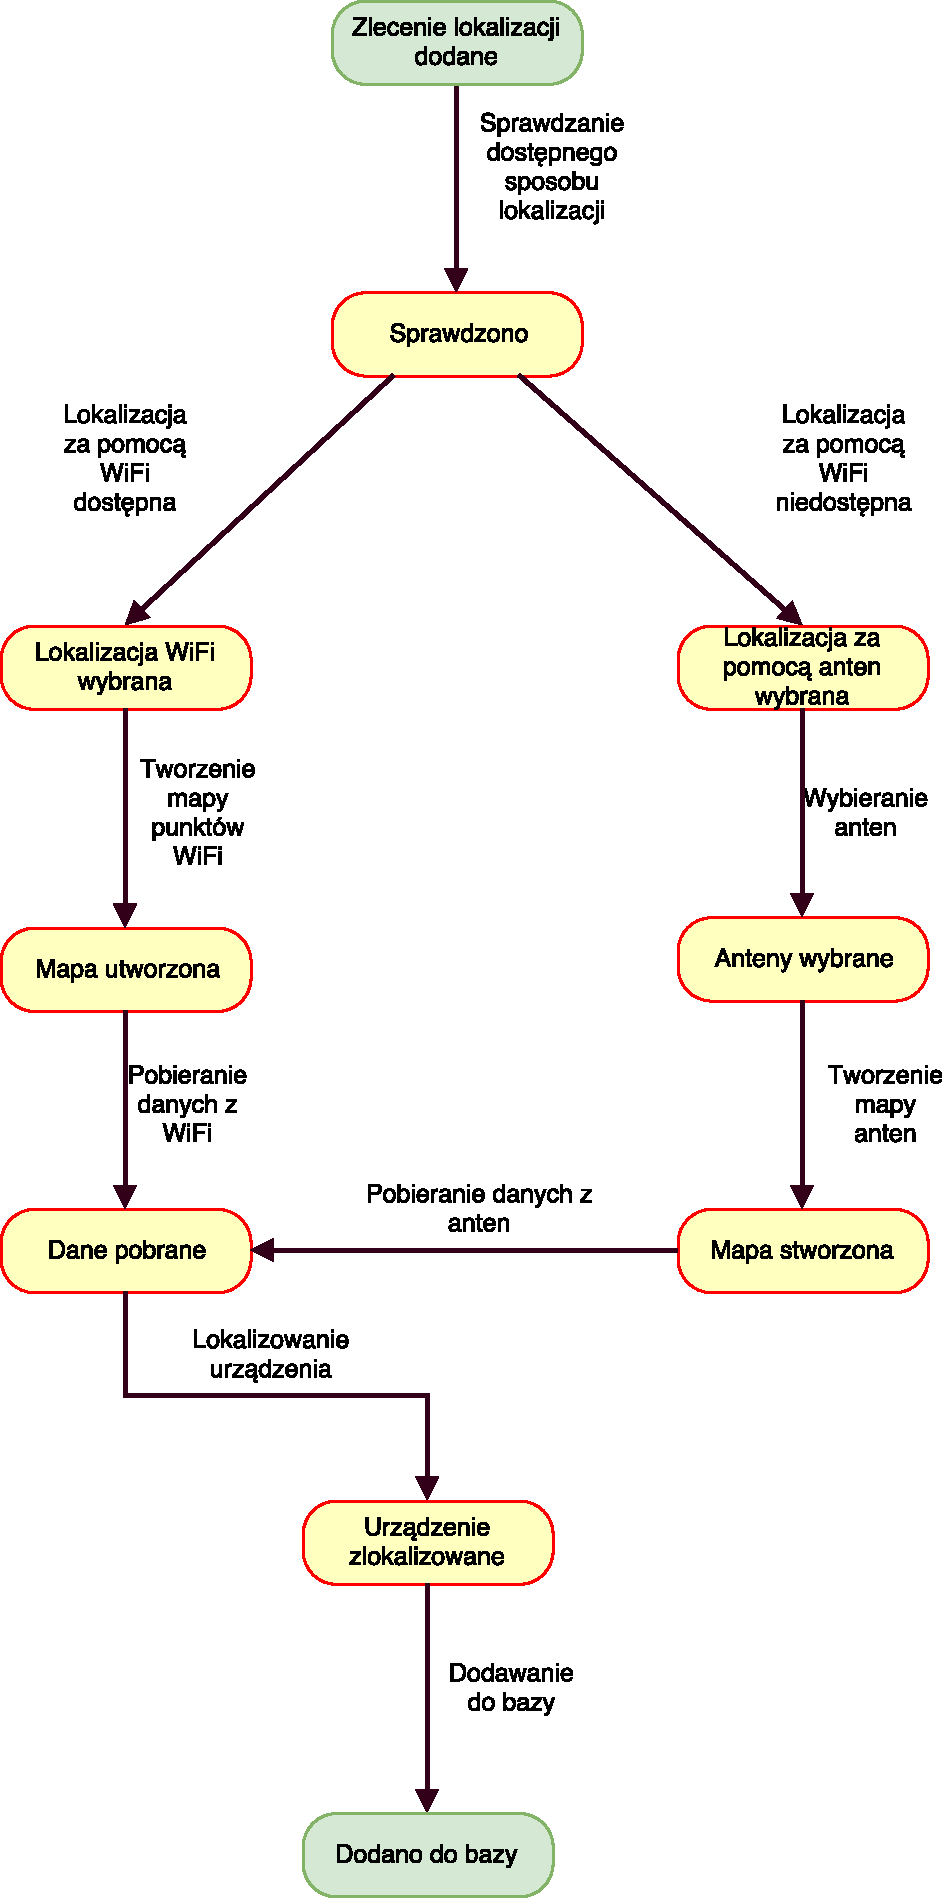
\includegraphics[scale=0.9]{STD1.pdf}
	\end{center}
	\newpage
	\subsection{STD poziom 1}
	\begin{center}
		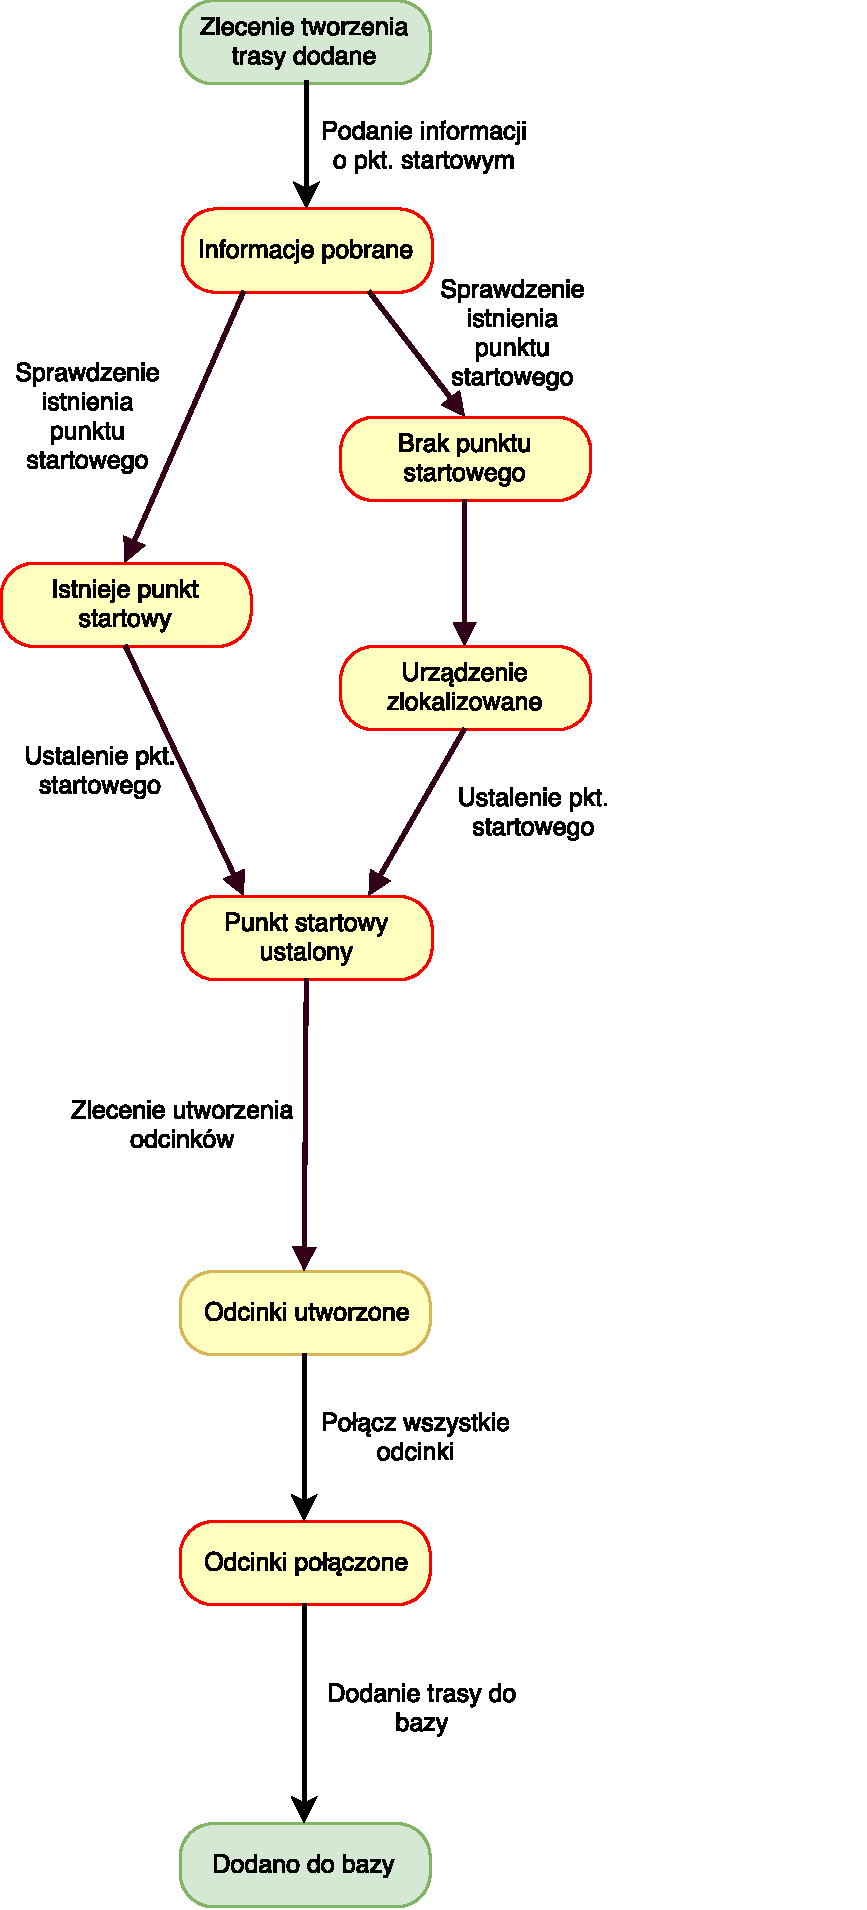
\includegraphics[scale=0.9]{STD2.pdf}
	\end{center}
	\newpage
	\subsection{STD poziom 1}
	\begin{center}
		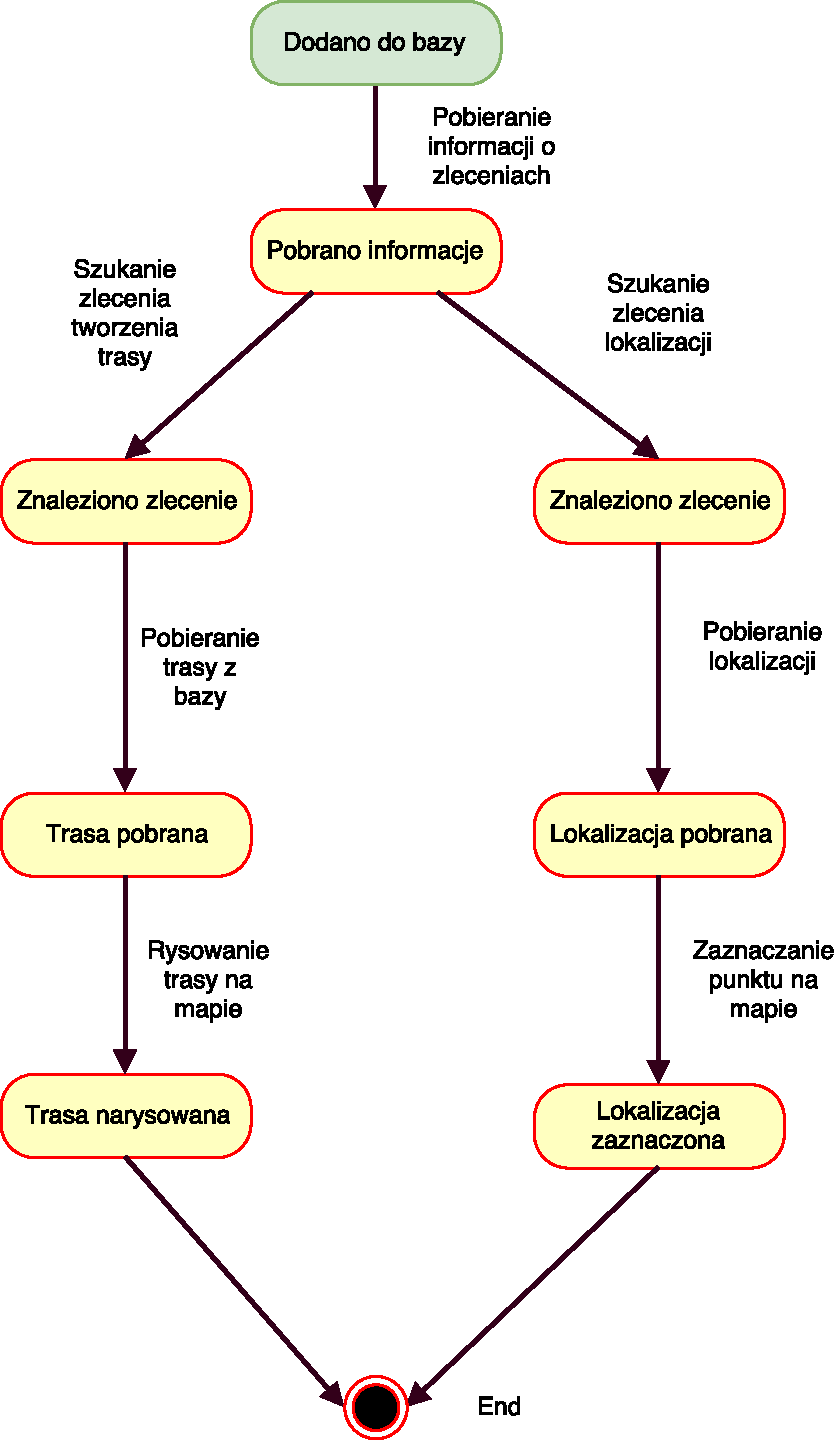
\includegraphics[scale=0.95]{STD3.pdf}
	\end{center}
	\newpage
	\subsection{STD poziom 2}
	\begin{center}
		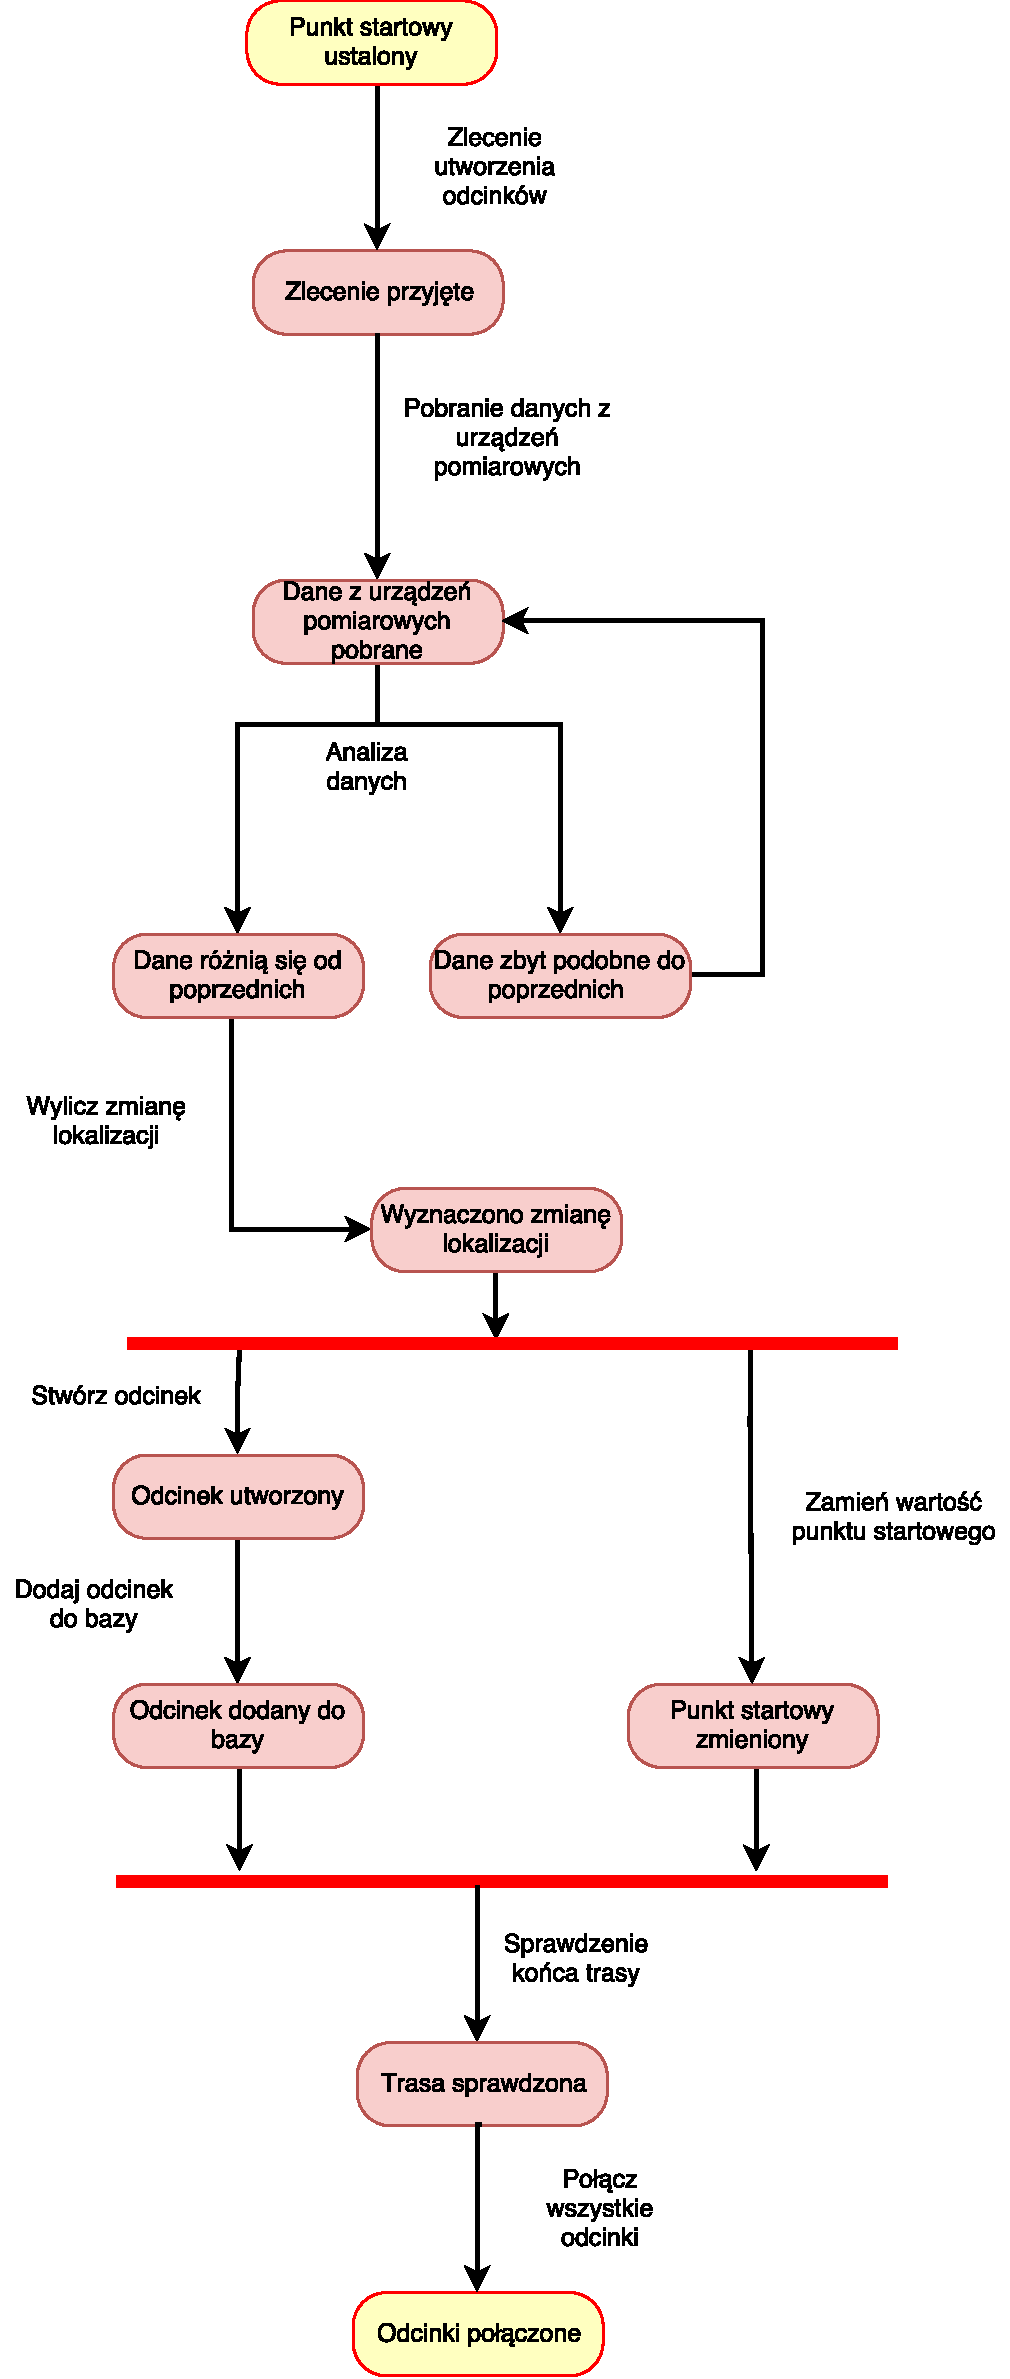
\includegraphics[scale=0.75]{STD4.pdf}
	\end{center}
\end{document}